\section{Parameters that Affect a Knowledge Graph Construction}
\label{chapter5:sec-param}
%Following the FAIR principles~\citep{wilkinson2016fair} and Open data initiatives, the size of publicly available data has grown exponentially in the last decade, expecting a faster growth rate in the following years as a result of the advances in the technologies for data generation and ingestion. In order to extract values for existing datasets, several data integration approaches have been proposed in the literature~\citep{Halevy18}. The Semantic Web community has also proposed various approaches that enable the integration  of data presented in diverse formats into a knowledge graph. Knowledge graphs comprise data and the knowledge that describe the main characteristics of the integrated data following a graph-based data model, e.g. RDF ~\citep{VidalEJSR19}. 
%With the aim of transforming structured data in tabular or nested formats like CSV, relational, JSON, and XML, into RDF knowledge graphs, diverse mapping languages have been proposed. Exemplary mapping languages include RDF Mapping Language (RML)~\citep{dimou2014rml}, R2RDF~\citep{sequeda2014obda}, xR2RML \citep{michel2015translation}, and R2RML~\citep{R2RML}, as well as tools like KARMA~\citep{GuptaSKGTM12}, SPARQL-Generate~\citep{lefranccois2017sparql}, and DIG~\citep{knoblock2015exploiting}.  
Despite these developments, the absence of testbeds has prevented the community from conducting fair evaluations of the existing tools for knowledge graph construction. This testbed deficiency has also impeded for a holistic understanding about the pros and cons of the state of the art, as well as for clear directions to advance the area. Given the expected growth rate of available data, testbeds are demanded in order to devise the next generation of tools able to integrate data at scale.

In this section, we study the process of knowledge graph construction and analyze various variables and configurations that can impact on the performance of materialization techniques. The relevant parameters studied in this work include selectivity of the joins between mapping rules, types of relations, and percentage of duplicates. We also present diverse examples that evidence the heterogeneous behavior that each engine may exhibit whenever small changes are conducted to the variables and the configurations of a testbed.  

We devise a set of parameters involved in a knowledge graph construction process and we empirically show how they can impact on the behavior of two existing engines: RMLMapper\footnote{\url{https://github.com/RMLio/rmlmapper-java}} and SDM-RDFizer\footnote{\url{https://github.com/SDM-TIB/SDM-RDFizer}}; these engines are compliant with the RML specification according to a set of defined test-cases\footnote{\url{http://rml.io/implementation-report/}}. We develop a synthetic data generator for the generation of (semi)-structured data and RML mapping rules, that consider the identified set of parameters. The results of our empirical study provide evidence of the importance of the proposed set of variables and configurations during the evaluation of these tools. The testbeds used to conduct this evaluation are available
online\footnote{\url{https://github.com/SDM-TIB/KGC-Param-Eval}}.

Our main contribution includes the definition of various dimensions and set of variables to be considered during the creation of testbeds or to be measured while the evaluation of knowledge graph construction tools. Another contribution represents the empirical evaluation of the effects that the variables and configurations have on the tasks of knowledge graph construction. Furthermore, the results of the experimental study contribute to the understanding of the pros and cons of the studied engines, and the directions that need to be followed in order to devise tools able to scale up to real-world scenarios.  

\subsection{Motivation Example}

We motivate our work by analyzing different scenarios where the performance of RMLMapper and SDM-RDFizer may be affected by changing the configuration of the testbeds utilized for empirically evaluating these engines. We aim at remarking the importance of taking into account different parameters during the definition of a testbed. We first describe a scenario where na\"ive parameters (size and format) leads to wrong decisions during the comparing of SDM-RDFizer and RMLMapper. The testbeds include a data source with one thousand rows, different number of predicate-object (POM) in RML triple maps, and diverse configurations of selectivity of triple map joins.

%\begin{figure}[t!]
%	\centering
%	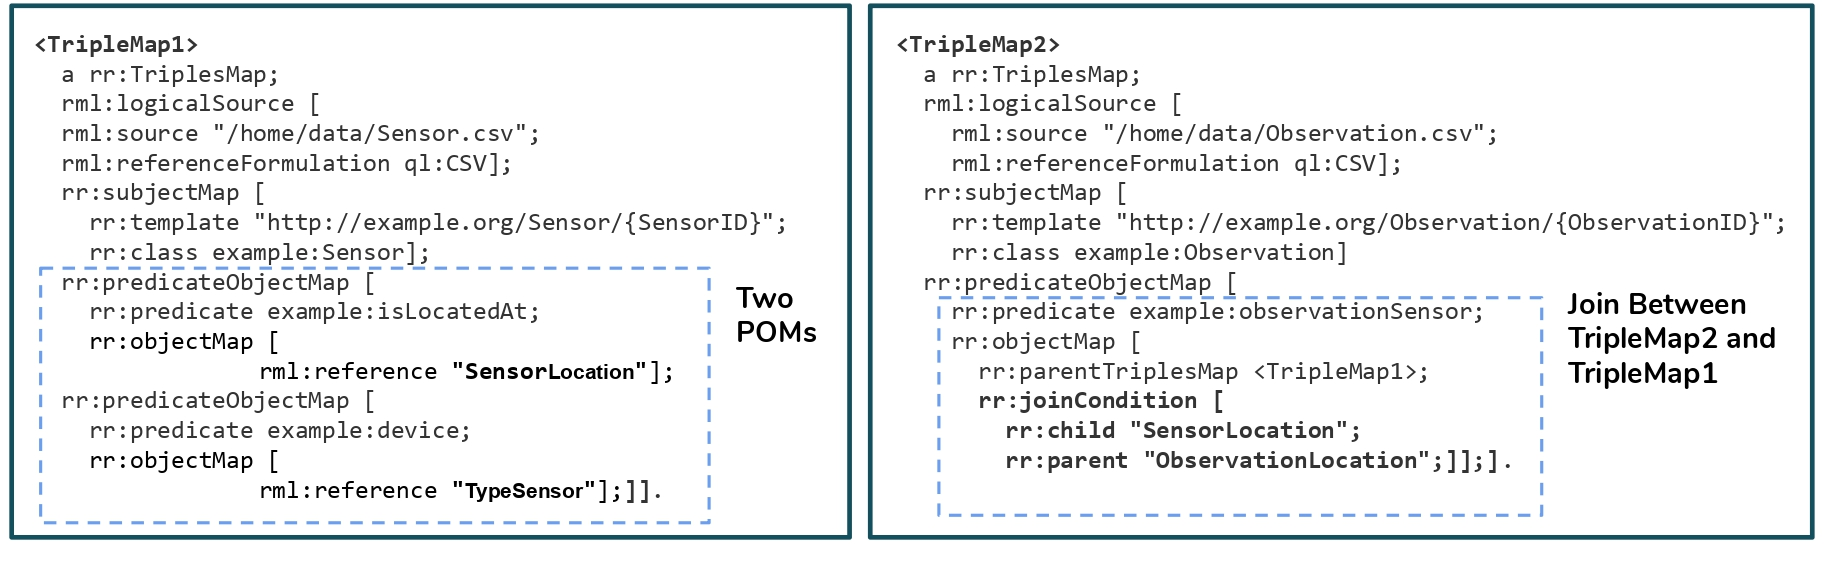
\includegraphics[width=\columnwidth]{figures/TripleMap.jpg}
%	\caption[RML Mapping example]{{\bf Motivating Example.} RML triple maps to transform two CSV files into RDF. TripleMap1 is composed of two predicate-object, i.e., Two POM. TripleMap2 has a join to TripleMap1; Observation.csv (outer relation) is joined to  Sensor.csv (inner relation) and the result, SensorID, is used as an object value.}
%	\label{fig:mappingRule}
%\end{figure}

%RML expresses mappings to transform sources represented in (semi)-structured format, e.g. CSV or XML, into RDF. Each mapping rule in RML, named RML triple map, is represented in RDF and consists of the following parts \citep{dimou2014rml}:
%\begin{itemize}
%    \item A \emph{Logical Source} that refers to a data source from where data is collected.
%    \item A \emph{Subject Map} that defines the subject of the generated RDF triples. 
%    \item \emph{Predicate-Object Maps} (POM) that expresses the predicate and the object the RDF triple to be generated; a triple map can comprise several POMs.
%\item
%A \emph{Referencing Object Map}, that indicates the reference or join condition to another triple map; the subject URL is the referenced triple map corresponds to the result of the evaluation of the join. 
%\end{itemize}
%\autoref{fig:mappingRule} illustrates two RML triple maps. \texttt{TripleMap1} is composed of two predicate-object maps, i.e. it is a Two POM mapping rule. \texttt{TripleMap2} has a referencing object map that joins the records of file Observation.csv with the records of the file Sensor.csv on the attributes \texttt{SensorLocation} and \texttt{ObservationLocation}. The result of executing the join between the two RML triple maps is the identifier of the sensor that collected the observation; this value is used as the object value of the predicate \texttt{observationSensor}.
%\subsubsection{Impact of Number of Predicates and Objects in Mapping Rules}
In this example, we execute a testbed where three different configurations of an RML mapping rule: Two-POM, Five-POM, and Ten-POM, i.e. they correspond to three mapping rules with two, five, and ten Predicate-Object Maps, respectively. 
Both engines exhibit a similar behavior while the number of predicate-object maps varies from two to five POMs, as shown in Table~\ref{tab:trivial}. However, when more complex mapping rules with more POMs are considered, the behavior of the SDM-RDFizer and RMLMapper is not impacted equally. Moreover, the results suggest that RMLMapper execution time increases with the number of POMs, while the SDM-RDFizer seems to be slightly affected. 
\begin{table}[ht!]
\centering
\caption[Impact of number of POMs on KGC engines]{\textbf{Impact of Number of Predicate-Object Maps.} Various predicate object maps (POM) specified in the mapping rules. The behavior of the two engines is similar when the mapping rules are simple (less than 5 POM) but it is different when more complex mappings are running (10 POM); time in seconds.
}
\label{tab:trivial}
\begin{tabular}{|l|c|c|}
\hline
\multicolumn{1}{|c|}{\multirow{2}{*}{\textbf{Engine}}} & \textbf{\begin{tabular}[c]{@{}c@{}}Execution \\ time (secs.)\end{tabular}} & \multicolumn{1}{l|}{\textbf{Number of results}} \\ \cline{2-3} 
\multicolumn{1}{|c|}{} & \multicolumn{2}{c|}{\textbf{Two POM}} \\ \hline
\multicolumn{1}{|c|}{\textbf{RMLMapper}} & 0.92  & 2,000 \\ \hline
\multicolumn{1}{|c|}{\textbf{SDM-RDFizer}} & 1.72 & 2,000 \\ \hline
\multicolumn{1}{|c|}{\textbf{}} & \multicolumn{2}{c|}{\textbf{Five POM}} \\ \hline
\textbf{RMLMapper} & 1.84 & 5,000 \\ \hline
\textbf{SDM-RDFizer} & 1.85 & 5,000 \\ \hline
 & \multicolumn{2}{c|}{\textbf{Ten POM}} \\ \hline
\textbf{RMLMapper} & 3.36 & 10,000 \\ \hline
\textbf{SDM-RDFizer} & 1.98 & 10,000 \\ \hline
\end{tabular}
\end{table}
%\subsubsection{Impact of Join Selectivity}
We now consider another parameter, the join selectivity, i.e. the cardinality of matching values from outer to the inner table (relation), in a referencing object map between two RML mapping rules. The join selectivity varies from 
\textbf{High Selectivity}, \textbf{Medium Selectivity}, and \textbf{Low Selectivity}, and Table~\ref{tab:joinSelectivity} reports on the results of RMLMapper and  SDM-RDFizer. First, it can be observed that the RMLMapper execution time increases by around $8$ seconds, while the SDM-RDFizer behavior is not equally affected by the selectivity of the join condition. As can be seen in Table~\ref{tab:joinSelectivity}, the SDM-RDFizer execution time (in seconds) increases from high to medium selectivity by $0.04$ (from $2.16$ to $2.20$), then decreases from medium to low selectivity by $0.01$ (from $2.20$ to $2.19$).
On the other hand, the RMLMapper execution time increases by $1.83$ (from $38.6$ to $40.43$), and $5.63$ (from $40.43$ to $46.06$) seconds from high to medium, and medium to low selectivity, respectively. As in the previous example, both engines are not equally affected by the complexity of the testbed. 

\begin{table}[ht!]
\centering
\caption[Impact of join selectivity on KGC engines]{\textbf{Impact of Join Selectivity.} Impact of the join selectivity variable over the engines with high, medium and low percentage of selectivity. While RMLMapper engine behavior increases in terms of execution time when the selectivity decreases, the SDM-RDFizer behavior is maintained, i.e. this variable affects to the first engine but it does not impact equality to the second one.}
\label{tab:joinSelectivity}
\begin{tabular}{|l|c|c|}
\hline
\multicolumn{1}{|c|}{\multirow{2}{*}{\textbf{Engine}}} & \textbf{\begin{tabular}[c]{@{}c@{}}Execution \\ time (secs.)\end{tabular}} & \multicolumn{1}{l|}{\textbf{Number of results}} \\ \cline{2-3} 
\multicolumn{1}{|c|}{} & \multicolumn{2}{c|}{\textbf{High Selectivity}} \\ \hline
\multicolumn{1}{|c|}{\textbf{RMLMapper}} & 38.6 & 2,100 \\ \hline
\multicolumn{1}{|c|}{\textbf{SDM-RDFizer}} & 2.16 & 2,100 \\ \hline
\multicolumn{1}{|c|}{\textbf{}} & \multicolumn{2}{c|}{\textbf{Medium Selectivity}} \\ \hline
\textbf{RMLMapper} & 40.43 & 23,000 \\ \hline
\textbf{SDM-RDFizer} & 2.20 & 23,000 \\ \hline
 & \multicolumn{2}{c|}{\textbf{Low Selectivity}} \\ \hline
\textbf{RMLMapper} & 46.06 & 30,000 \\ \hline
\textbf{SDM-RDFizer} & 2.19 & 30,000 \\ \hline
\end{tabular}
\end{table}

The uncorrelated behavior of studied engines shows clearly the need to considering diverse variables and configurations during the definition of testbeds, and thus, uncovering characteristics of these engines. In this work, we analyze the parameters that might affect a knowledge graph construction process and evaluate some of the most problematic ones (e.g. partitioning, relation type) to remark the importance of setting them during testbed design.  
 
\subsection{Relevant Parameters for Testbed Design}

{\small
\ctable[
	cap     = Variables and configurations that impact on KGC engines,
	caption =  \textbf{Variables and Configurations}. Set of variables and configurations that impact on the behavior of the tools for knowledge graph creation. Independent variables are divided into five groups and the impact on the observed variables is depicted., topcap,
	label   = {table:variables},
	maxwidth= 1.0\textwidth,
	pos = hb!,
]
%{c l c | c | c}
{X X c | c }
{
}{
\FL
% 
& &\multicolumn{2}{c}{\textbf{Observed Variables}}\NN
%\cmidrule(){3-5}
%   
\multicolumn{2}{c}{\multirow{2}{*}{ {\bf Independent Variables}}}  \\
%\multicolumn{2}{c}{ Observed Variables} &  Hidden Variables\\
\cmidrule(){3-4}
&	   & Execution Time & Completeness \ML
\multirow{10}{*}{\textbf{Mapping}}
        & mapping order				& \checkmark & \\
		& \# triplesMap 					& \checkmark & \checkmark  \\
		& \# predicateObjectMaps				& \checkmark & \checkmark \\ 
		& \# predicates				& \checkmark &\checkmark \\ 
		& \# objects				& \checkmark & \checkmark\\ 
		& \# joins				& \checkmark & \checkmark \\ 
		& \# named graphs				& \checkmark & \checkmark \\ 
		& join selectivity				& \checkmark & \checkmark \\  
		& relation type				& \checkmark & \checkmark \\ 
		& object TermMap type 			& \checkmark &        \ML
\multirow{5}{*}{\textbf{Data}}
        &  dataset size & \checkmark &                     		 \\
		&  data frequency distribution			& \checkmark &     \\
		&  type of partitioning		&   \checkmark                   & \checkmark  \\
		% &  \# sources		&   \checkmark                   &   \\
		&  data format 		& \checkmark & \checkmark  \ML
\multirow{3}{*}{\textbf{Platform}}
		&  cache on/off 				&      \checkmark              &   \\
		&  RAM available 				&         \checkmark            &    \\
		&  \# processors				&         \checkmark            &    
		\ML		
\multirow{3}{*}{\textbf{Source}}
		& distribution data transfer 					& \checkmark & \checkmark  \\
		& initial delay 					& \checkmark &   \\
		& access limitation     		      & \checkmark & \checkmark  
		\ML	
		%&  Sponge parameter	&    		      & \checkmark & \checkmark 
%
\multirow{3}{*}{\textbf{Output}}
		&  Serialization 				&      \checkmark              & \checkmark   \\
		&  Duplicates 				&         \checkmark            & \checkmark   \\
		&  Generation type				&         \checkmark            & \checkmark  
		\ML	
}
}

In this section, we perform a study of the parameters that have impact on the knowledge graph construction engines. First, we identify the generic groups of parameters involved and the effect they produce in this process. Second, we provide a list of specific variables that influence the construction of knowledge graphs and determine the relationships among them. Finally, we describe each parameter in detail given the reasons why it might affect the performance of the engines. Together with these descriptions, we provide use cases over a set of parameters to illustrate the importance of involving them in a testbed definition.

As in every empirical study, we consider two groups of variables: independent and observed. The independent variables are those features that need to be specified in a benchmark to ensure that the performed evaluation is reproducible. These variables are grouped in five dimensions: mapping, data, platform, source, and output.
On the other hand, observed variables correspond to those characteristics that are measured during the evaluation of the testbed and that may be influenced by independent variables. The observed variables are as follows:
\begin{itemize}
    \item \textit{Execution time:} The variable is in turn comprised of: \textit{i) Time for the first triple} (elapsed time between the engine starts and the first triple), \textit{ii) total execution time} required to produce all the triples of the knowledge graph.
    \item \textit{Completeness:} Number of returned triples in relation to all the RDF triples that should be created according to the data and input mappings.
\end{itemize}
The relations among independent and observed variables are presented in Table \ref{table:variables}. These variables are described in detail in the next section. 


\subsubsection{Mapping Dimension}
This dimension involves the variables that characterise the mappings in terms of their structure and evaluation. Regarding the structure, there are various aspects to be considered: mapping order, the complexity of the mapping in terms of number of predicates, objects, and the join type and selectivity.

\noindent \textbf{Mapping Order.} Although the mappings are usually defined using an RDF serialisation, where the order is not relevant, the features of each \texttt{rr:tripleMap} (e.g. joins) can affect the execution plan generated by each tool, having, thus, a potential negative impact on the total execution time.


\begin{table}[ht!]
\centering
\caption[Impact of relation types on KGC engines]{\textbf{Impact of Relation types.} Various relation types in a join specified in the mapping rules. N corresponds to 15 values in the case of 1-N and N-1 relations, N and M has 10 values in the last case. RMLMapper execution time is not affected by 1-N and N-1 relation types while it is affected by  N-M relations. SDM-RDFizer performs better in N-1 than 1-N but the time increases in N-M.}
\label{tab:relationType}
\begin{tabular}{|l|c|c|}
\hline
\multicolumn{1}{|c|}{\multirow{2}{*}{\textbf{Engine}}} & \textbf{\begin{tabular}[c]{@{}c@{}}Execution \\ time (secs.)\end{tabular}} & \multicolumn{1}{l|}{\textbf{Number of results}} \\ \cline{2-3} 
\multicolumn{1}{|c|}{} & \multicolumn{2}{c|}{\textbf{1-1}} \\ \hline
\multicolumn{1}{|c|}{\textbf{RMLMapper}} & 42.86 & 25,000 \\ \hline
\multicolumn{1}{|c|}{\textbf{SDM-RDFizer}} & 2.19 & 25,000 \\ \hline
\multicolumn{1}{|c|}{\textbf{}} & \multicolumn{2}{c|}{\textbf{1-N}} \\ \hline
\textbf{RMLMapper} & 43.34 & 22,490 \\ \hline
\textbf{SDM-RDFizer} & 2.19 & 22,490 \\ \hline
\textbf{} & \multicolumn{2}{c|}{\textbf{N-1}} \\ \hline
\textbf{RMLMapper} & 43.26 & 22,490 \\ \hline
\textbf{SDM-RDFizer} & 2.15 & 22,490 \\ \hline
 & \multicolumn{2}{c|}{\textbf{N-M}} \\ \hline
\textbf{RMLMapper} & 78.64 & 25,200 \\ \hline
\textbf{SDM-RDFizer} & 2.33 & 25,200 \\ \hline
\end{tabular}

\end{table}

\noindent \textbf{Mapping complexity.} The number of properties defined in a rule mapping, e.g. number of predicates, objects, or named graphs may affect the observed variables because the number of triples to be generated, is related to what is specified in the mappings. Additionally, the \texttt{rr:termtype} of the \texttt{rr:objectMap} can affect the total execution time because the cost of generating a constant or a template is not the same. Finally, the join selectivity and types of relation have also impact on the performance of an engine. In Table \ref{tab:relationType}, we illustrate how the relation type affects the total execution time of the studied engines. In this case, the behavior of the RMLMapper only occurs when the relation type is N-M. However, the SDM-RDFizer behavior is impacted during the evaluation of 1-N and N-M joins. Additionally, during the join evaluation, there are many cases when duplicates are generated, then the engines have to eliminate them. Table \ref{tab:duplicates} reports on how the generation of the duplicates --during the join condition evaluation-- affects the total execution time. RMLMapper decreases its performance while the percentage of duplicates increases. However,  SDM-RDFizer implements optimised data structured that allow for efficiently eliminating duplicates, and seems not to be equally affected by the complexity of these configurations, e.g. number of duplicates. 

\begin{table}[!tb]
\centering
\caption[Impact of duplicates on KGC engines]{\textbf{Impact of duplicates generation during join evaluation.} Various configurations of duplicates generated during the evaluation of a join between two triple maps. While the complexity of the configuration increases (more percentage of duplicates), the RMLmapper decreases its performance. Surprisingly, the SDM-RDFizer seems not to be affected by the complexity of the testbeds, and improves its performance even when the complexity of testbeds increases.}
\label{tab:duplicates}
\begin{tabular}{|l|c|c|}
\hline
\multicolumn{1}{|c|}{\multirow{2}{*}{\textbf{Engine}}} & \textbf{\begin{tabular}[c]{@{}c@{}}Execution \\ time (secs.)\end{tabular}} & \multicolumn{1}{l|}{\textbf{Number of results}} \\ \cline{2-3} 
\multicolumn{1}{|c|}{} & \multicolumn{2}{c|}{\textbf{Low percentage of duplicates}} \\ \hline
\textbf{RMLMapper} & 37.94 & 20,027 \\ \hline
\textbf{SDM-RDFizer} & 2.01 & 20,027 \\ \hline
\multicolumn{1}{|c|}{\textbf{}} & \multicolumn{2}{c|}{\textbf{Medium percentage of duplicates}} \\ \hline
\textbf{RMLMapper} & 39.201 & 20,105 \\ \hline
\textbf{SDM-RDFizer} & 1.87 & 20,105 \\ \hline
\textbf{} & \multicolumn{2}{c|}{\textbf{High percentage of duplicates}} \\ \hline
\textbf{RMLMapper} & 40.81 & 20,263 \\ \hline
\textbf{SDM-RDFizer} & 1.89 & 20,263 \\ \hline
\end{tabular}
\end{table}

\subsubsection{Data Dimension}
We describe the independent variables related with the original data that are required for the generation of a knowledge graph. Each dataset can be defined in terms of \textbf{size} and \textbf{total number of sources}. The first characteristic impacts on the number of triples that will be generated, affecting, thus, the total execution time. Additionally, the total number of sources that have to be processed to generate a knowledge graph may also affect the total execution time.

\noindent \textbf{Partitioning} and \textbf{distribution} are important variables considered in the construction of a knowledge graph. Partitioning refers to the way that a dataset is fragmented, and distribution is the format (e.g. CSV, JSON) of each partition. A dataset can be presented in only one format or in multiples formats, and this variable affects not only the total execution time but also the completeness of the results. A dataset may be fragmented into disjointed partitions; the partition may be horizontal, vertical or a combination of both. Horizontal partitioning fragments the dataset, so that, they represent different instances of the same resource (equal \textit{TripleMaps} with different sources). Vertical partitioning produces fragments that contain at least one property of the same resources (\textit{TriplesMaps} with \textit{JoinCondition}). The horizontal partitioning may affect the completeness of a knowledge graph while the vertical partitioning has an influence on the execution time. Table \ref{tab:partitioning} compares the behavior of the RMLMapper and SDM-RDFizer with different configurations. The two engines increase their execution time when the horizontal partitioning is compared with and without including replication. However, RMLMapper decreases its execution time when the vertical partitions with and without replication are compared, while SDM-RDFizer execution time increases.  Thus, even SDM-RDFizer is tailored towards efficient duplicate elimination, data partitioning-- with and without replication -- seems to affect the SDM-RDFizer performance. \newline

% Please add the following required packages to your document preamble:
% \usepackage{multirow}
\begin{table}[!tb]
\centering
\caption[Impact of partitioning on KGC engines]{\textbf{Impact of Partitioning}: Various configurations of vertical and horizontal partitioning with and without duplicates. The two engines perform similar with the two cases of the horizontal partitioning but they have different behaviors in vertical partitioning.}
\label{tab:partitioning}
\begin{tabular}{|l|c|c|}
\hline
\multicolumn{1}{|c|}{\multirow{2}{*}{\textbf{Engine}}} & \textbf{\begin{tabular}[c]{@{}c@{}}Execution \\ time (secs.)\end{tabular}} & \textbf{Number of results} \\ \cline{2-3} 
\multicolumn{1}{|c|}{} & \multicolumn{2}{c|}{\textbf{Horizontal Partitioning without Replication}} \\ \hline
\textbf{RMLMapper} & 1,904.31 & 310,000 \\ \hline
\textbf{SDM-RDFizer} & 4.84 & 310,000 \\ \hline
\multicolumn{1}{|c|}{\textbf{}} & \multicolumn{2}{c|}{\textbf{Vertical Partitioning without Replication}} \\ \hline
\textbf{RMLMapper} & 2,067.77 & 310,000 \\ \hline
\textbf{SDM-RDFizer} & 4.73 & 310,000 \\ \hline
\textbf{} & \multicolumn{2}{c|}{\textbf{Horizontal Partitioning with Replication}} \\ \hline
\textbf{RMLMapper} & 2,276.98 & 310,000 \\ \hline
\textbf{SDM-RDFizer} & 5.86 & 310,000 \\ \hline
\textbf{} & \multicolumn{2}{c|}{\textbf{Vertical Partitioning with Replication}} \\ \hline
\textbf{RMLMapper} & 2,024.66 & 310,000 \\ \hline
\textbf{SDM-RDFizer} & 4.98 & 310,000 \\ \hline
\end{tabular}
\end{table}

\subsubsection{Platform Dimension}
The platform dimension comprises variables related with the hardware used to create a knowledge graph. We include a set of variables related with the system cache, the available RAM memory for running the tool, and the number of processors of the machine. The \textbf{cache} and the \textbf{available RAM memory} may affect the total time execution.  We recommend that other parameters, like the versions of operating system and processor, should be specified in the evaluation setup. To conclude, during testbed design, the platform and hardware specification requires attention and  needs to be defined in detail.

\subsubsection{Source Dimension}
In this dimension, we consider different variables related with the original sources defined in the mapping rules. The \textbf{distribution data transfer}, which corresponds to the transfer time of a file by a Web service--in case the data is not in a local machine-- will definitely influence the total execution time. Additionally, the \textbf{initial delay} of each engine to configure the corresponding wrappers for each data format and the \textbf{limit access} for example, a database, also strikes out the execution time and the completeness of the results.

\subsubsection{Output Dimension}
In this dimension, we consider the variables related with the output of the generation process. The \textbf{serialization} impacts on the total execution time; the effect will depend on the size of the output and the number of times the processor has to access the disk to store the output. \textbf{Generation type} represents how an engine constructs a knowledge graph. The generation can be continuous, e.g. the SDM-RDFizer stores each RDF triple in a file once it is generated. Contrary, the generation can be in-memory, e.g. RMLMapper stores the output when the knowledge graph is created completely. Finally, the engines usually can have a flag for removing \textbf{duplicates}; this operation has to be specified in the setup because it strikes out the completeness and also the total execution time. The efficiency of the engines components that eliminate duplicates, can be captured by observing the variables of this dimension.   

As can be observed in the results reported in this section, the behavior of the studied engines is not equally affected by the different independent variables. Thus, benchmarks need to include all these variables in order to provide a holistic overview of the performance of the studied engines, and ensure general and reproducible evaluations. 


\subsection{Evaluation of affected parameters in KGC}
The goal of our experiment is to assess the impact of the discussed variables and configurations during the evaluation of existing knowledge graph creation tools. We aim at answering the following research questions: \textbf{RQ1}:What is the effect of mixing different variables in one testbed?; \textbf{RQ2}: What is the impact of considering configurations of different complexity of the same variable in one testbed?; \textbf{RQ3}: Do the different variables and configurations influence in the behavior of existing knowledge graph creation tools? To answer these research questions, we set up the following experimental studies:

\noindent \textbf{Datasets.}
For this evaluation, we generated three different datasets with 1,000 (1K), 10,000 (10K), and 50,000 (50K) rows, and various number of columns based on the tested parameters; ~\autoref{tab:datasets} shows the properties of the datasets generated for \texttt{Relation Type}, \texttt{Join Duplicates}, and \texttt{Join Selectivity} evaluations. 
For the \textit{Dataset Size (N{\"a}ive)} parameter, we generated the same number of rows as in~\autoref{tab:datasets}, but with $30$ columns.
\begin{table}[!tb]
    \centering
    \caption[Evaluated datasets]{\textbf{Datasets.} Properties of Datasets used in the Empirical Evaluations.}
    \label{tab:datasets}
    \begin{tabular}{|c|c|c|c|}
    \hline
     Dataset & \#rows & \#columns & \#tables \\ \hline
     1K & 1,000 & 2 & 2 \\ \hline 
     10K & 10,000 & 2 & 2 \\ \hline 
     50K & 50,000 & 2 & 2 \\ \hline 
     \end{tabular}
\end{table}
%
During the experiments, we only considered the CSV file format to represent the generated tables.

\begin{figure}[!tb]
    \centering
    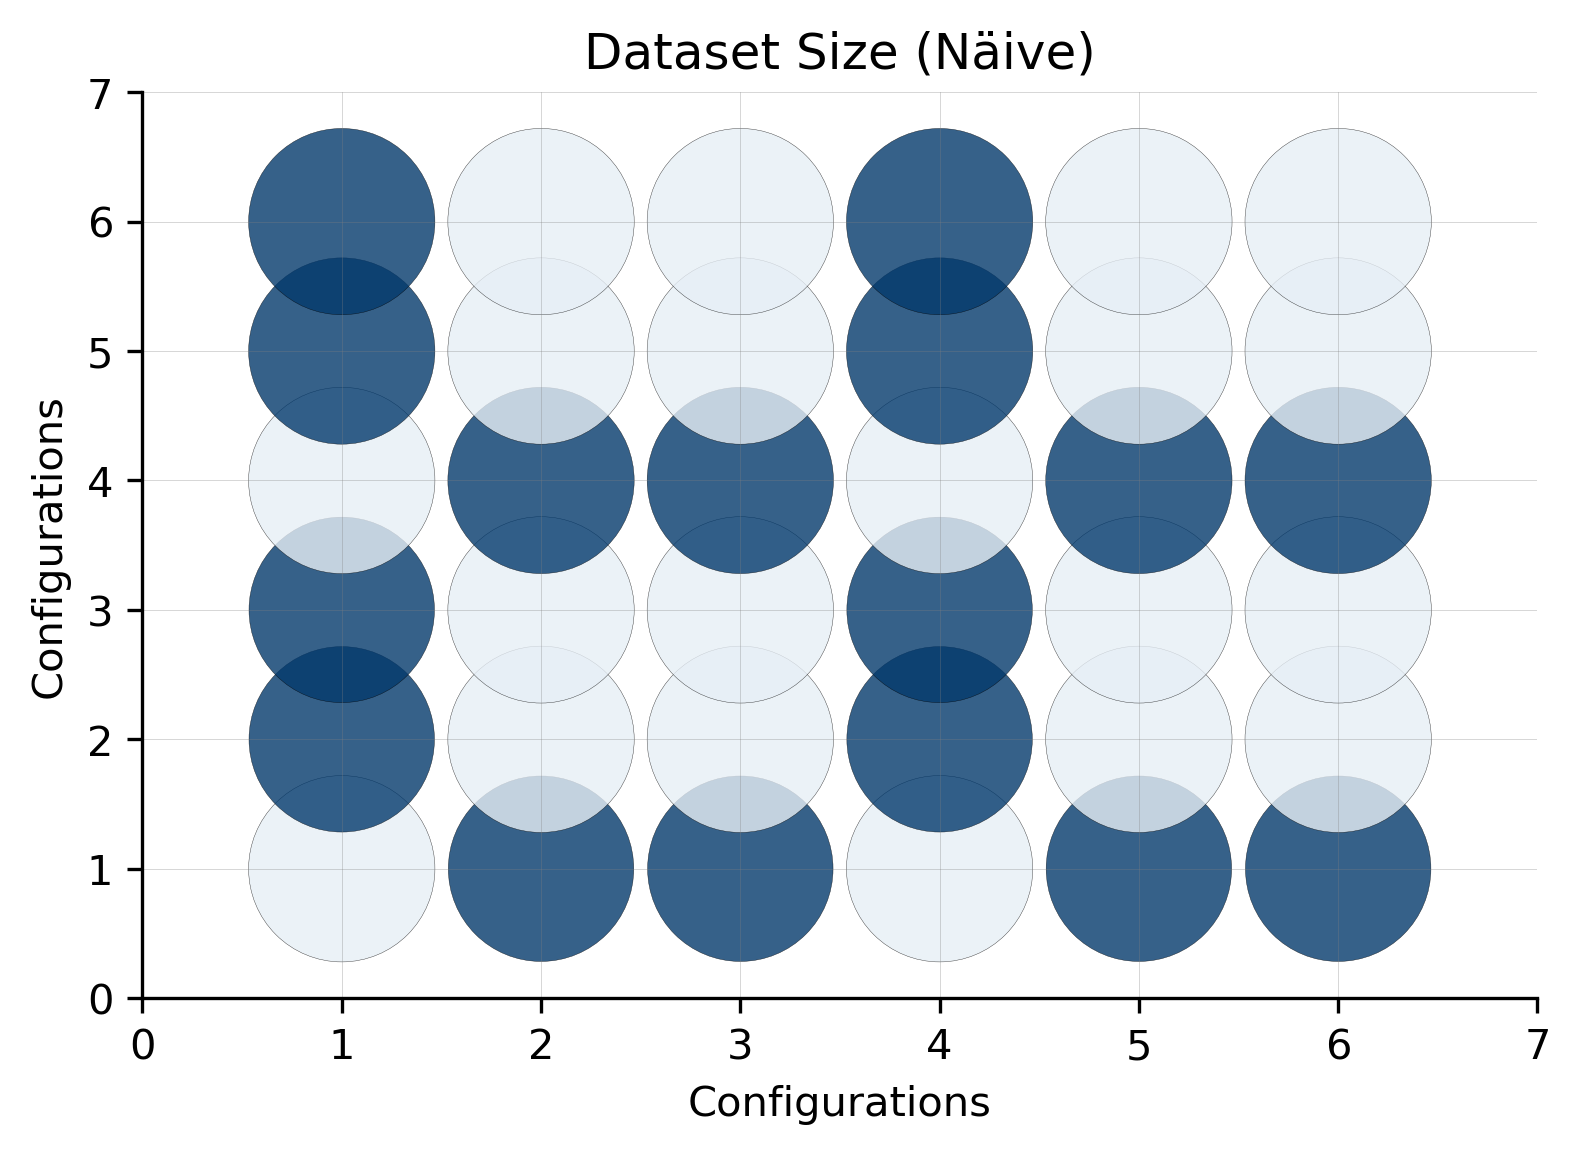
\includegraphics[width=0.8\columnwidth]{figures/naive_allk_bubble.png}
    \caption[Knowledge Graph Creation Tool on Different Dataset Sizes (Na{\"i}ve)]{\textbf{Comparison of Knowledge Graph Creation Tool on Different Dataset Sizes (Na{\"i}ve).} The first three configurations, i.e. 1, 2, and 3 in x-axis and y-axis, correspond to SDM-RDFizer on datasets 1K, 10K, and 50K, respectively. The last three configurations, i.e. 4, 5, and 6 on x-axis and y-axis, correspond to RMLMapper 1K, 10K, and 50K, respectively. Grey bubbles correspond to correlation value of $1.0$; blue bubbles show a positive correlation. The number of blue bubbles suggests that both systems exhibit similar behavior.}
    \label{fig:naive_bubble}
\end{figure}

\noindent \textbf{Configurations.}
We consider different configurations for the above-discussed variables in each dimension. 
%
\texttt{Dataset Size Configurations:} 1) SDM-RDFizer 1K; 2) SDM-RDFizer 10K; 3) SDM-RDFizer 50K; 4) RMLMapper 1K; 5) RML\-Mapper 10K; and 6) RMLMapper 50K. In each configuration of this parameter, we only use one data file.
%
\texttt{Relation Type configurations:} 1) SDM-RDFizer 1-N; 2) SDM-RDFizer N-1; 3) SDM-RDFizer N-M; 4) SDM-RDFizer Combinations (all relation types); 5) RMLMapper 1-N; 6) RMLMapper N-1; 7) RMLMapper N-M; and 8) RMLMapper Combinations (all relation types). For relation cardinality, we evaluated $N=\{1, 5, 10, 15\}$ and $M=\{1, 3, 5, 10\}$. In addition, we set the percentage of rows that involve in those relation types to $25\%$, i.e. $25\%$ of the overall rows from outer table have a matching join value to inner table, and $50\%$, respectively.
%
\texttt{Join Duplicate configurations:}  1) SDM-RDFizer Low, 2) SDM-RDFizer High, 3) RMLMapper Low, 4) RMLMapper High. \texttt{Low} Join Duplicates refer to datasets with low percentage of duplicates, i.e. from $5\%$ to $20\%$ of data generated could have duplicates due to the join conditions, similarly 
\texttt{High} Join Duplicates refer to higher percentage of duplicates, i.e. from $30\%$ to $50\%$ of data generated could be duplicated. 
%
\texttt{Join Selectivity Configurations:} 1) SDM-RDFizer High; 2) SDM-RDFizer Low; 3) RMLMapper High; and 4) RMLMapper Low. In this case, the join selectivity \texttt{High} represents how many time the join condition matches the values in the inner join file from 5\% to 20\% of the overall rows, while \texttt{Low} means that the join condition matches range from 60\% to 100\% of the overall number of rows. As previously shown, we hypothesise that these configurations allow us to uncover patterns in the behavior of these engines that could not be observed if only na{\"i}ve variables were studied. 

\noindent \textbf{Metrics}
We report on the following metrics or observed variables: 
\textit{Execution Time}: Elapsed time between execution of an engine and the delivery of the results.
\textit{Number of Results}: Number of triples generated by the KGC engine.

\noindent \textbf{Implementations.} 
The SDM-RDFizer and the testbeds are implemented in Python 3.6; the SDM-RDFizer is publicly available\footnote{\url{https://github.com/SDM-TIB/SDM-RDFizer}}. Furthermore, Jupiter Notebooks are available to generate the data and plot the results. Additionally, we have created a Docker image to run the testbeds and reproduce the experimental results\footnote{\url{https://github.com/SDM-TIB/KGC-Param-Eval}}. The experiments were run in an Intel(R) Xeon(R) equipped with a CPU E5-2603 v3 @ 1.60GHz 20 cores, 100G memory with Ubuntu 16.04LTS.


\begin{figure}[!tb]
    \centering
    \subfloat[Dataset 1K]{
      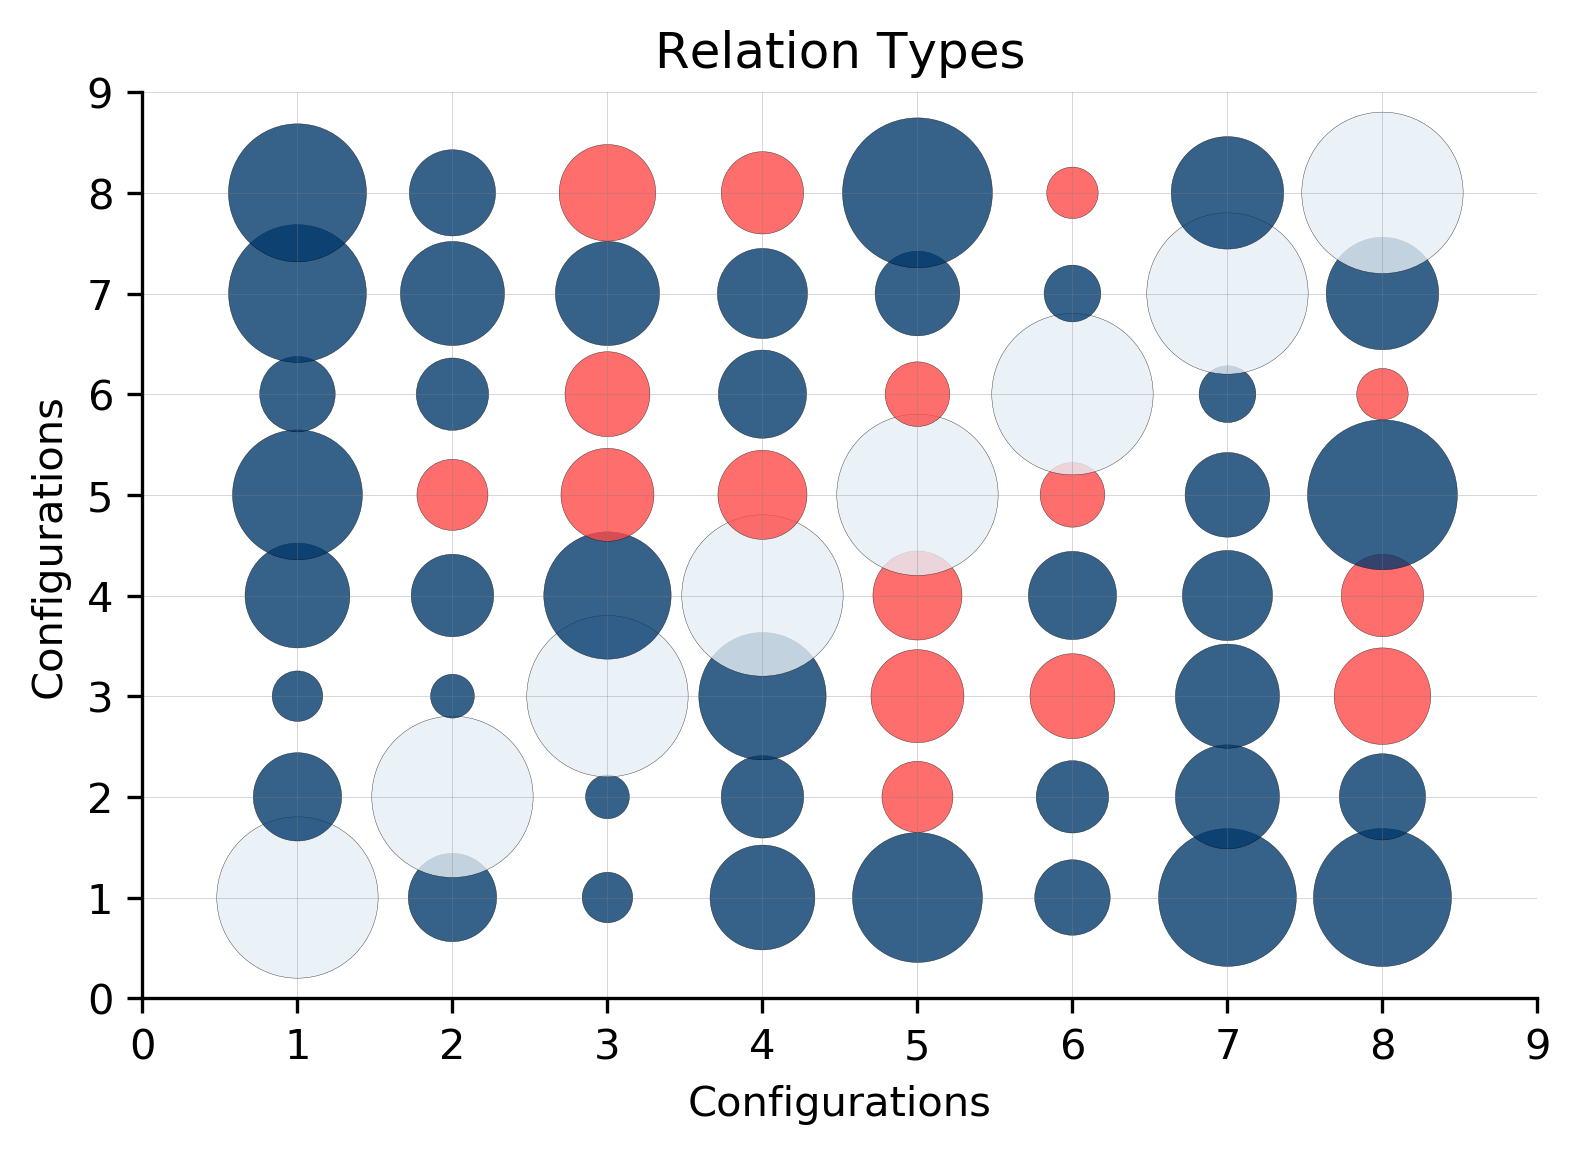
\includegraphics[width=0.48\columnwidth]{figures/relation_type_01k_bubble.png}
      \label{fig:rt_1k}
    }
    \subfloat[Dataset 10K]{
      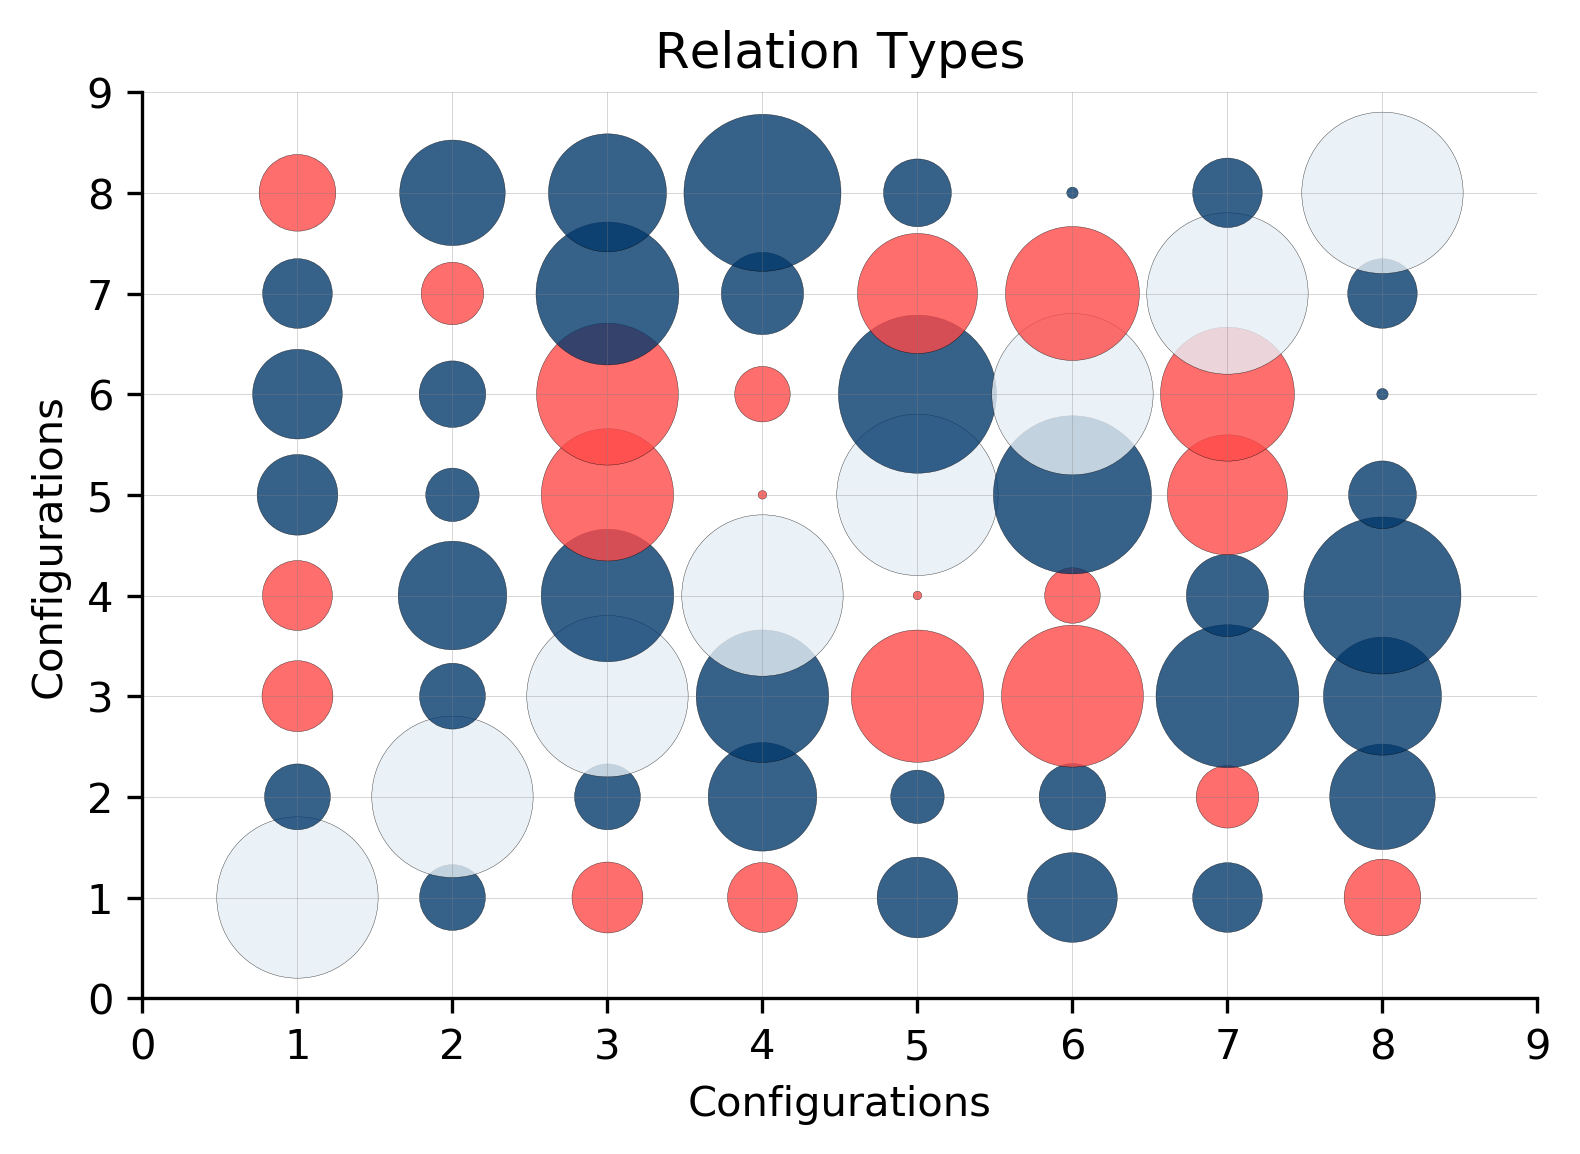
\includegraphics[width=0.48\columnwidth]{figures/relation_type_10k_bubble.png}
      \label{fig:rt_10k}
    }
    \qquad
    \subfloat[Dataset 50K]{
      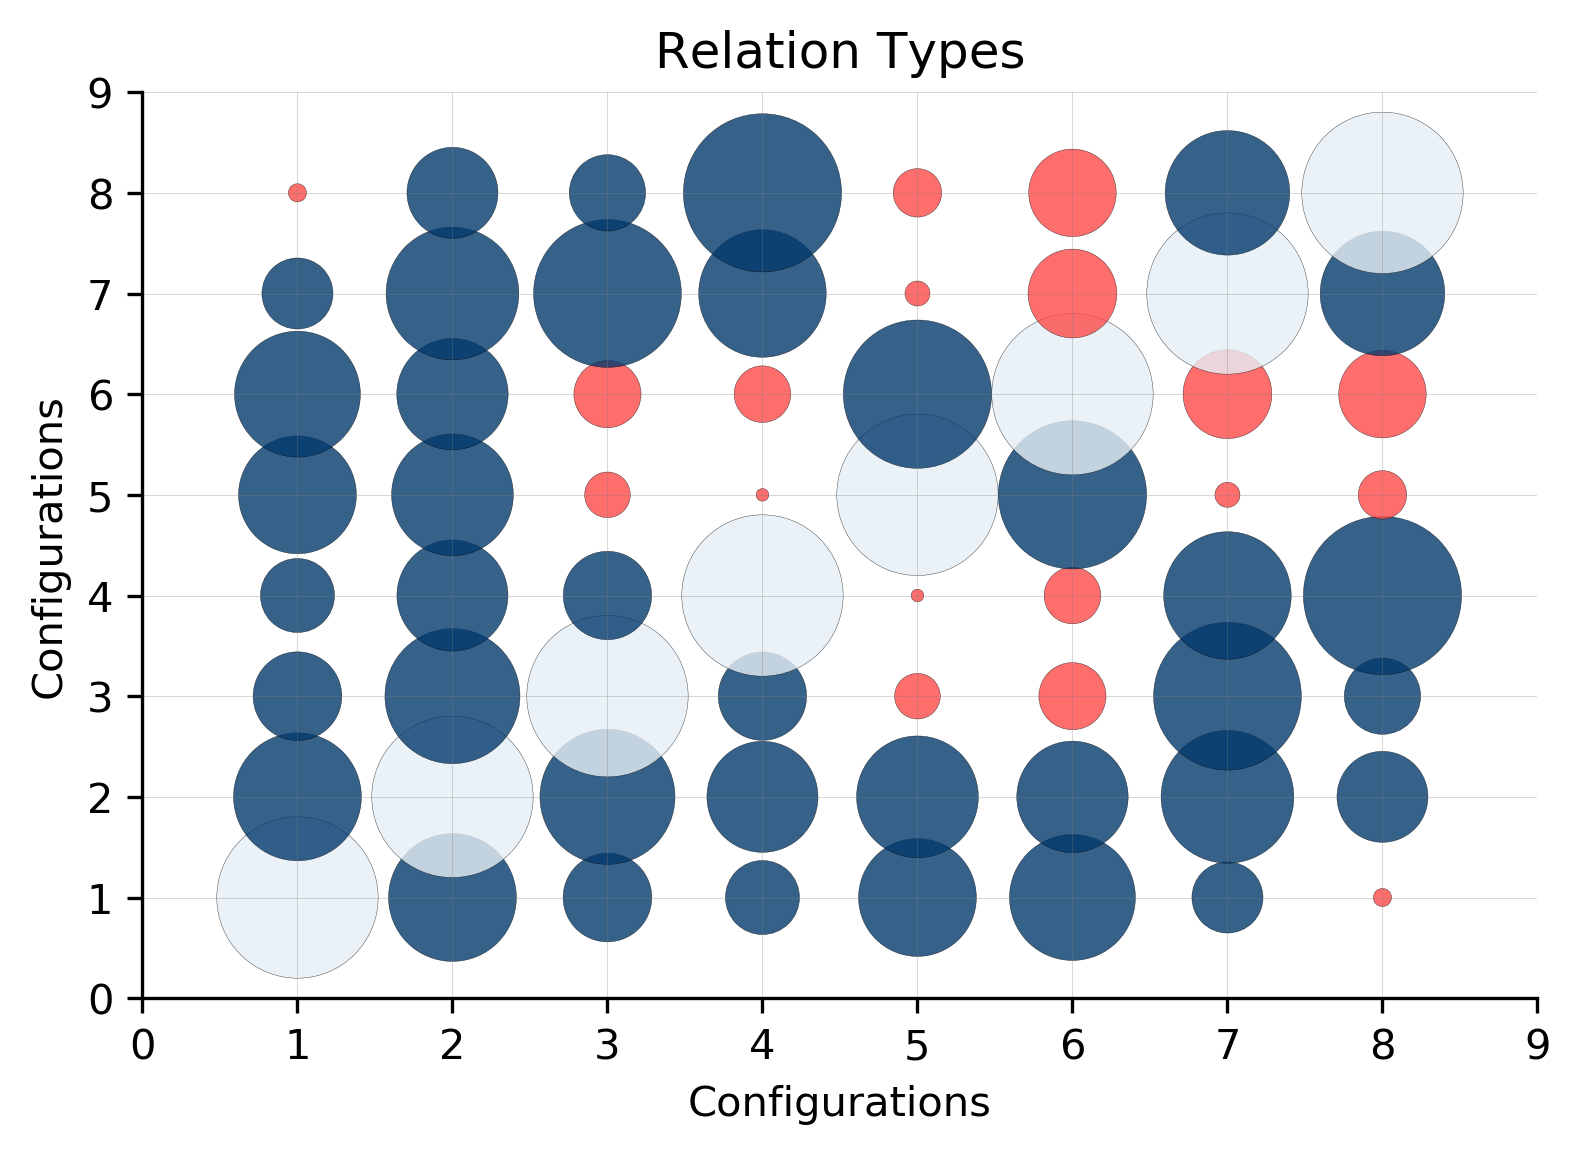
\includegraphics[width=0.48\columnwidth]{figures/relation_type_50k_bubble.png}
      \label{fig:rt_50k}
    }
    \subfloat[Combination of 1K, 10K, and 50K]{
      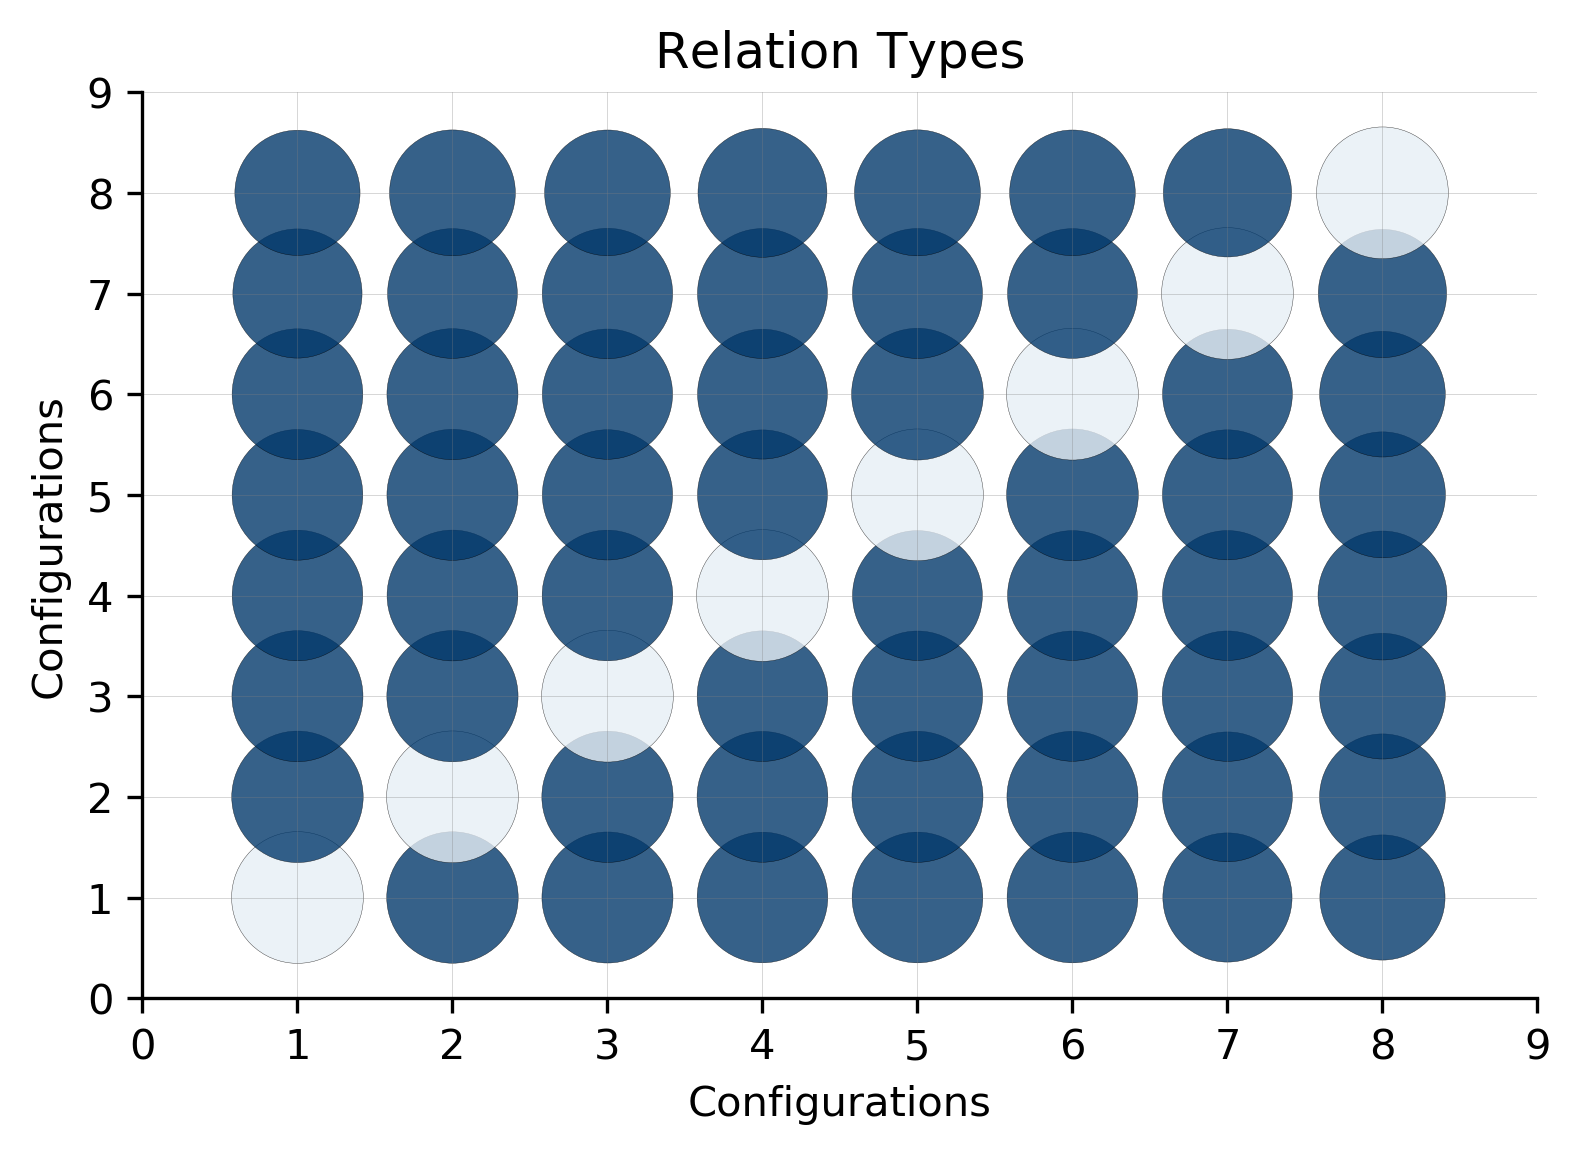
\includegraphics[width=0.48\columnwidth]{figures/relation_type_allk_bubble.png}
      \label{fig:rt_all}
    }
    \caption[Knowledge Graph Creation Tools on Different Types of Relations]{\textbf{Comparison of Knowledge Graph Creation Tools on Different Types of Relations.} The first four (4) configurations, i.e. 1-4 in both x-axis and y-axis, represent results of SDM-RDFizer on \textit{1-N}, \textit{N-1}, \textit{N-M}, and combination of all relations types, respectively. The later configurations, 5-8 both in x-axis and y-axis, shows results of RMLMapper on \textit{1-N}, \textit{N-1}, \textit{N-M}, and combination of all relations types, respectively. Grey bubbles correspond to correlation value of $1.0$; blue bubbles show a positive correlation while red bubbles show a negative correlation. The plots reveal that both type of relations and size of the dataset need to be taken into account to uncover patterns in the behavior of the engines. 
    }
    \label{fig:relation_type_bubble}
\end{figure}


\noindent \textbf{Testbeds.}
Results of each configurations are ordered from lower to higher complexity and compared using the Pearson's correlation. 
A high positive value of correlation between two configurations indicates that the corresponding engines had a similar behavior, i.e. the trends of execution time of the tools are similar; they are represented with blue bubbles in our plots. When a configuration is compared to itself, the Pearson's correlation reaches the highest value ($1.0$), represented with grey bubbles in our plots. 
On the other hand, a negative value indicates that there is an inverse correlation between the engines, i.e. they exhibit an opposite behavior; they are represented with red bubbles.


\subsubsection*{Discussion of the Observed Results}
We observe that the behavior of the engines can be affected when multiple variables are involved in a testbed (e.g. size and relation type) or when different levels of complexity of a variables (e.g. low, high join selectivity). We discuss the obtained results during our evaluation over the different configurations and parameters involved in each experiment:   

\noindent \textbf{Dataset Size (Na{\"i}ve):}
Figure~\ref{fig:naive_bubble} depicts the comparison of engines when the dataset size is considered. When \texttt{configuration 1} is compared to itself, the Pearson's correlation value is $1.0$; additionally, it is high and positive when it is compared to \texttt{configurations 2, 3, 5, and 6} (large blue bubbles). 
Using this parameter, the correlation analysis suggests that both engines behave similarly in all configurations. Moreover, this indicates that only considering the data size is not enough to uncovered the properties of the studied engines.


\begin{figure}[!tb]
    \centering
    \subfloat[Dataset 1K]{
      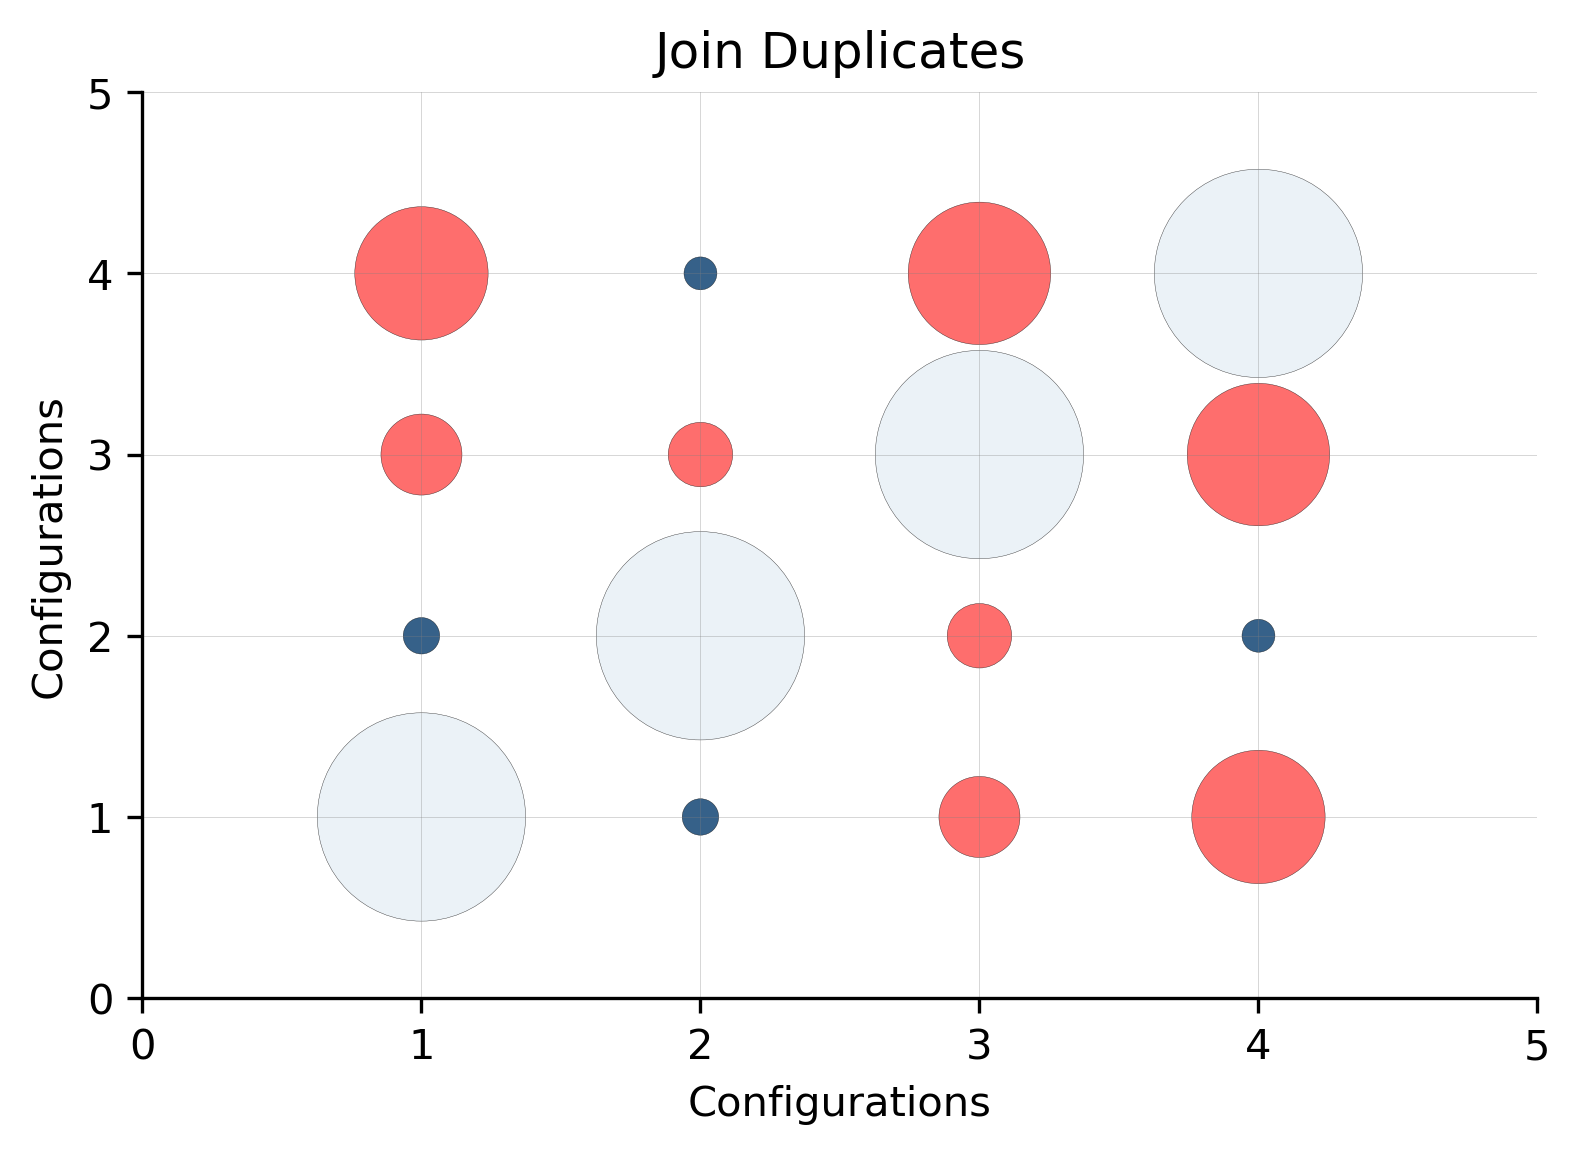
\includegraphics[width=0.48\columnwidth]{figures/duplicate_joins_01k_bubble.png}
      \label{fig:naive1}
    }
    \subfloat[Dataset 10K]{
      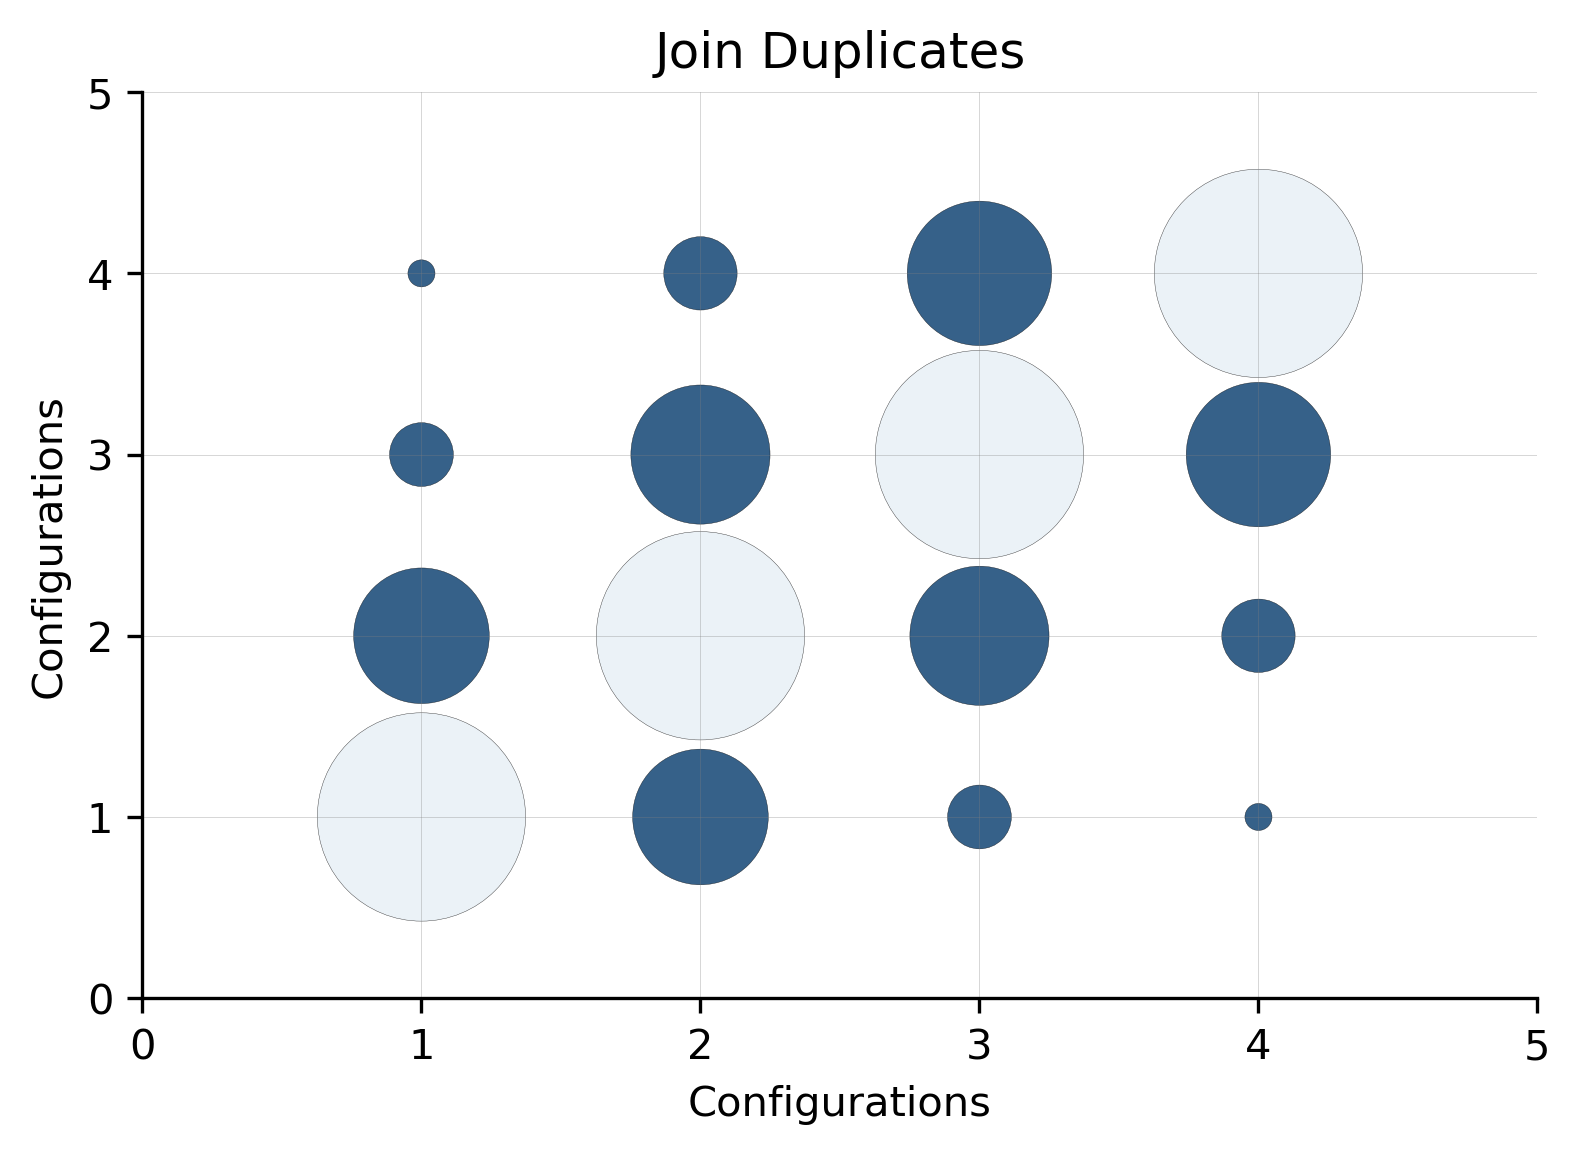
\includegraphics[width=0.48\columnwidth]{figures/duplicate_joins_10k_bubble.png}
      \label{fig:js0}
    }
    \qquad
    \subfloat[Dataset 50K]{
      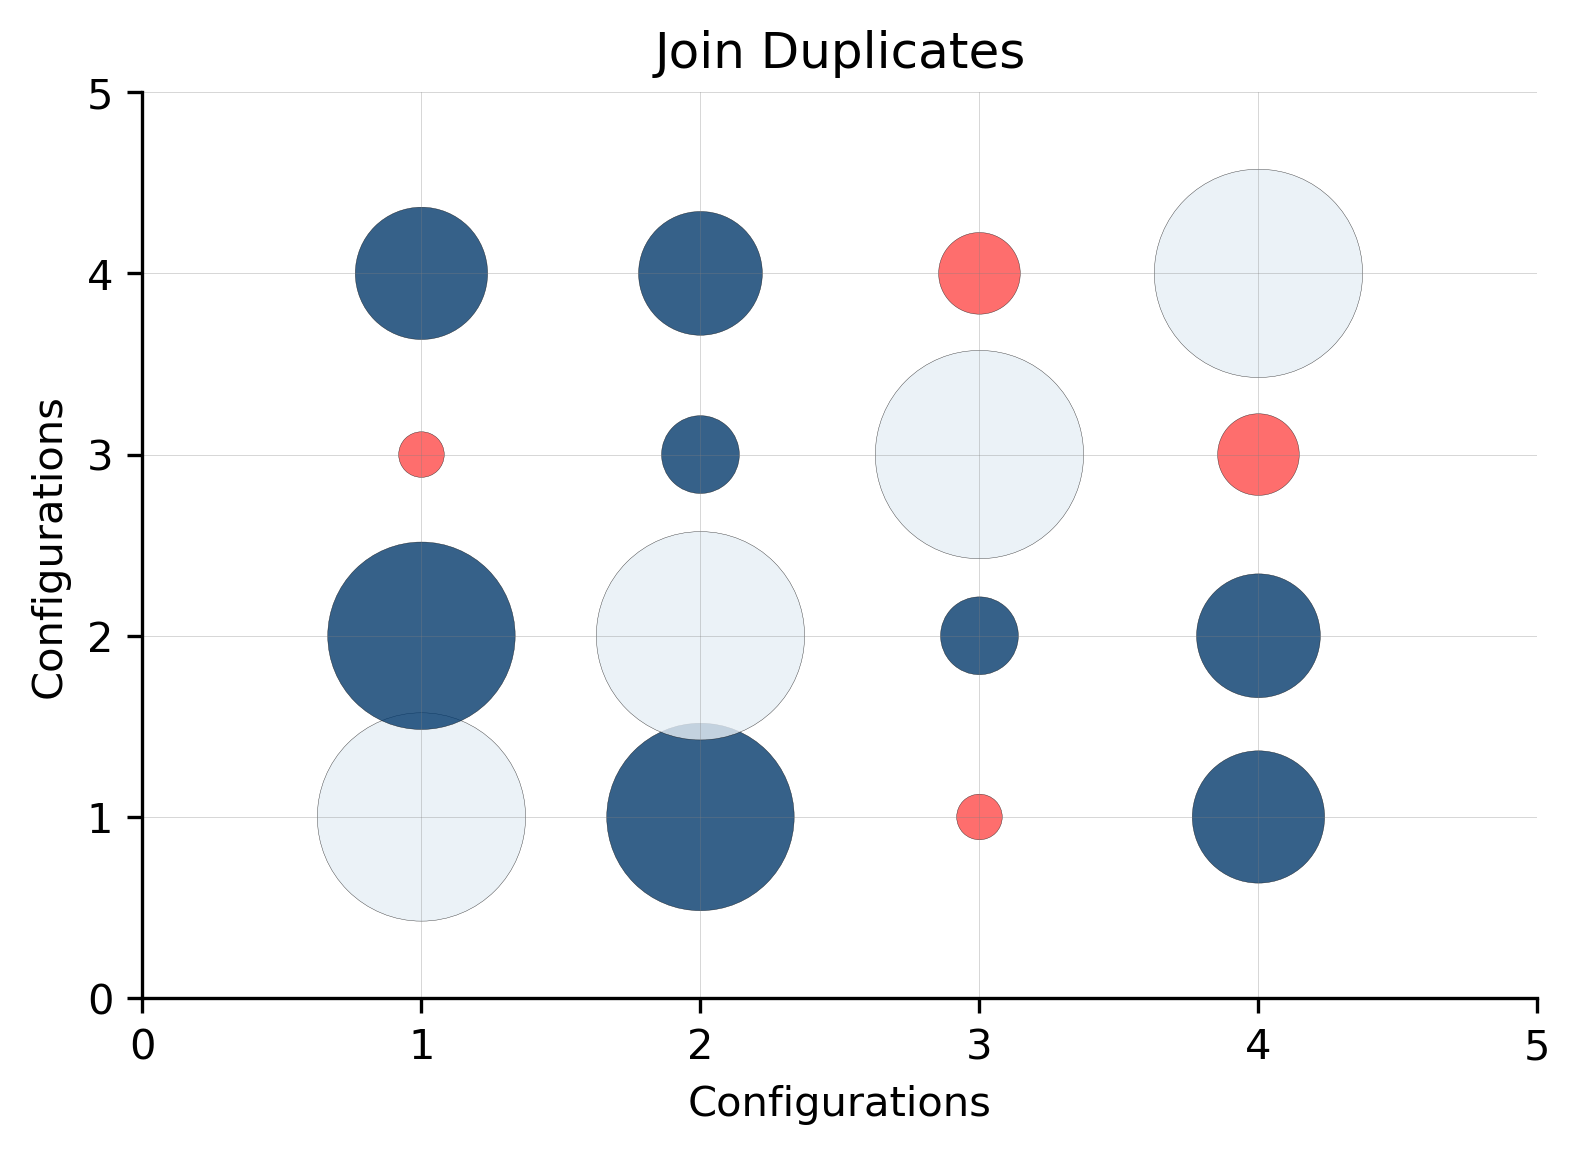
\includegraphics[width=0.48\columnwidth]{figures/duplicate_joins_50k_bubble.png}
      \label{fig:naive2}
    }
    \subfloat[Combination of 1K, 10K, and 50K]{
      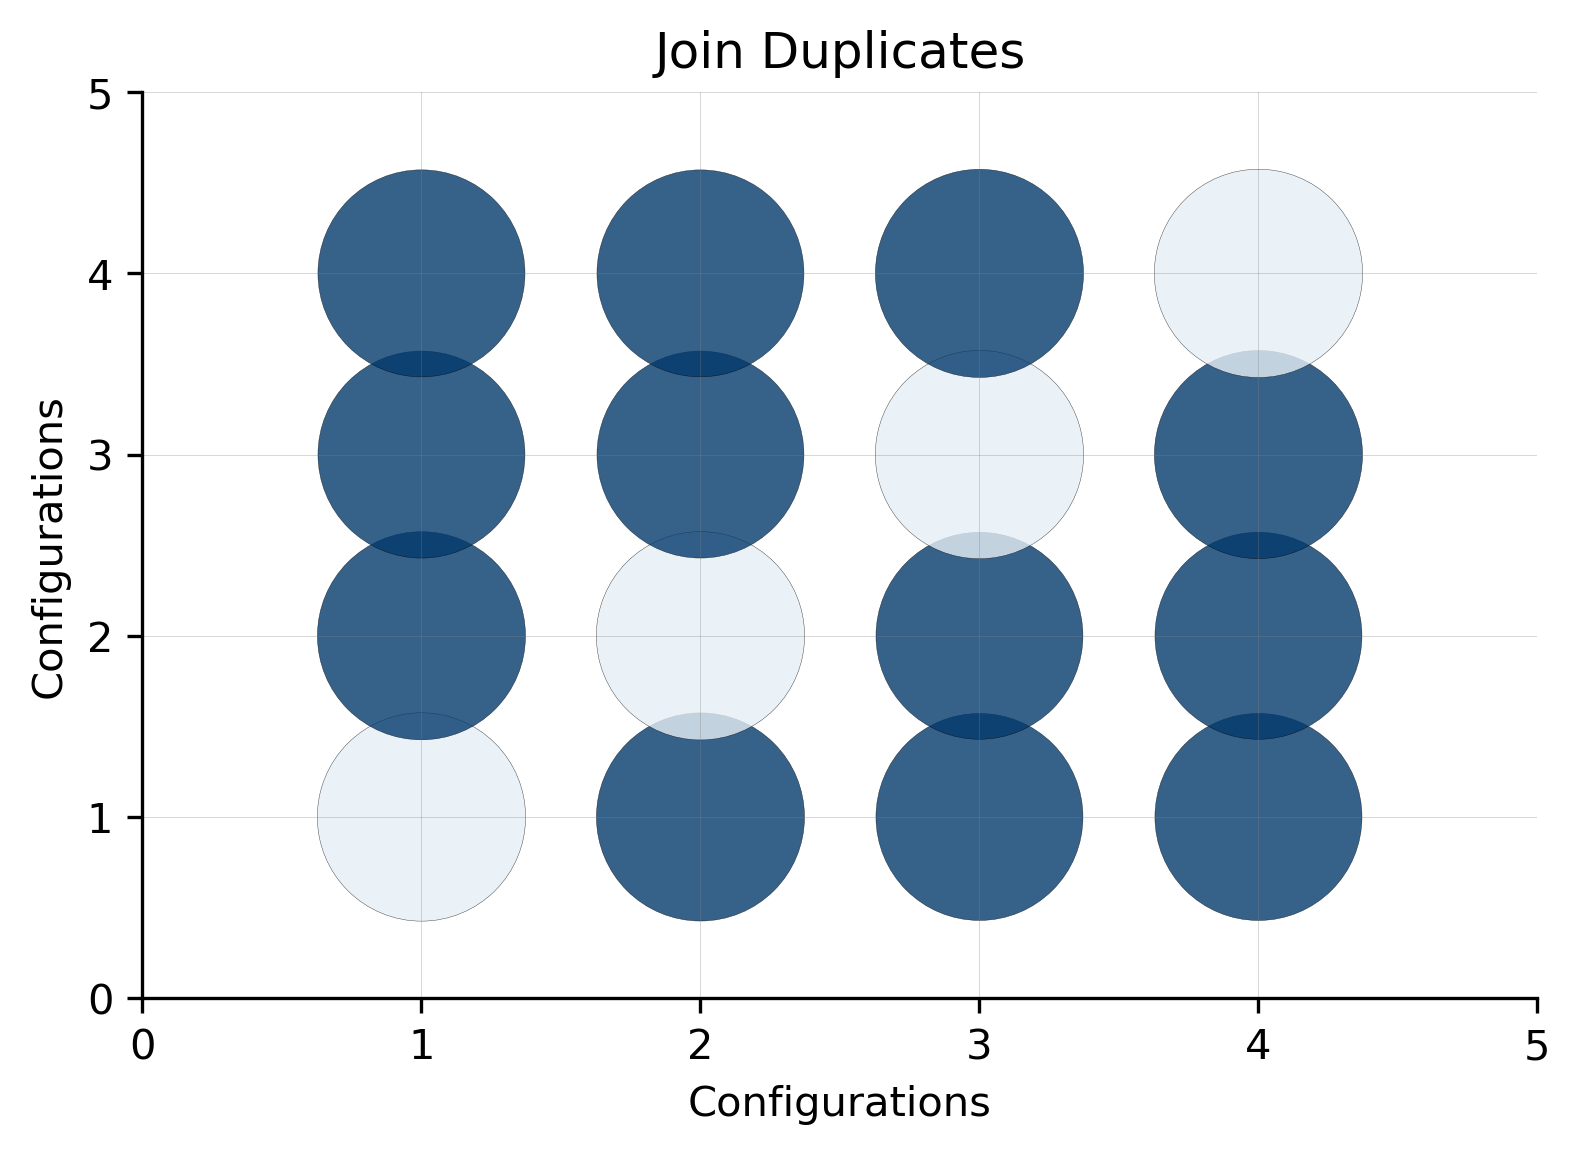
\includegraphics[width=0.48\columnwidth]{figures/duplicate_joins_allk_bubble.png}
      \label{fig:js1}
    }
    \caption[Knowledge Graph Creation Tools on Duplicates during Join]{\textbf{Comparison of Knowledge Graph Creation Tools on Duplicates during Join.} The first two (2) configurations, i.e., 1-2 on x-axis and y-axis, represent results of SDM-RDFizer on datasets with \textit{low} (5\%-20\% of data) number of duplicates and \textit{high} (30\%-50\% of data) number of duplicates generated during joins, respectively. The last two configurations, i.e., 3-4 on x-axis and y-axis, represent results of RMLMapper on datasets with \textit{low} number of duplicates and \textit{high} number of duplicates generated during joins, respectively. Grey bubbles correspond to correlation value of $1.0$; blue bubbles show a positive correlation while red bubbles show a negative correlation. Results evidence that both join duplicates and dataset size are needed for characterising an engine performance.}
    \label{fig:duplicates_bubble}
\end{figure}


\begin{figure}[!tb]
    \centering
    \subfloat[Dataset 1K]{
      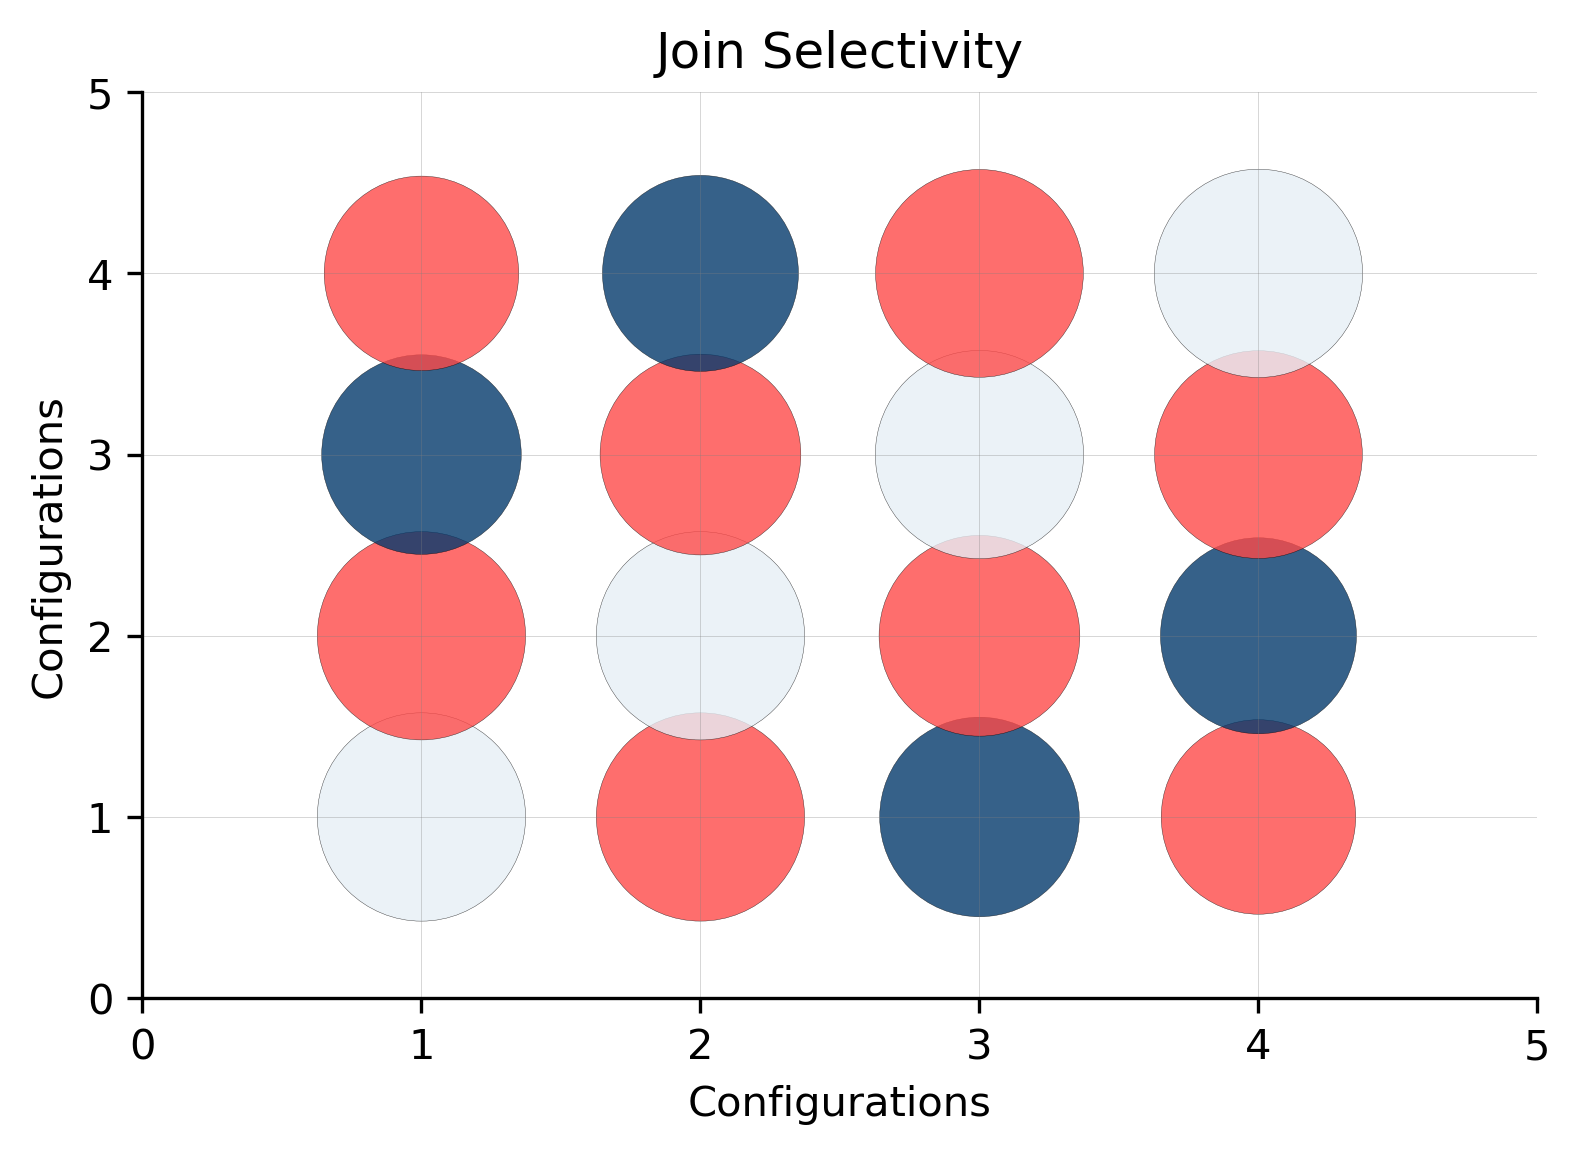
\includegraphics[width=0.48\columnwidth]{figures/join_selectivity_01k_bubble.png}
      \label{fig:naive3}
    }
    \subfloat[Dataset 10K]{
      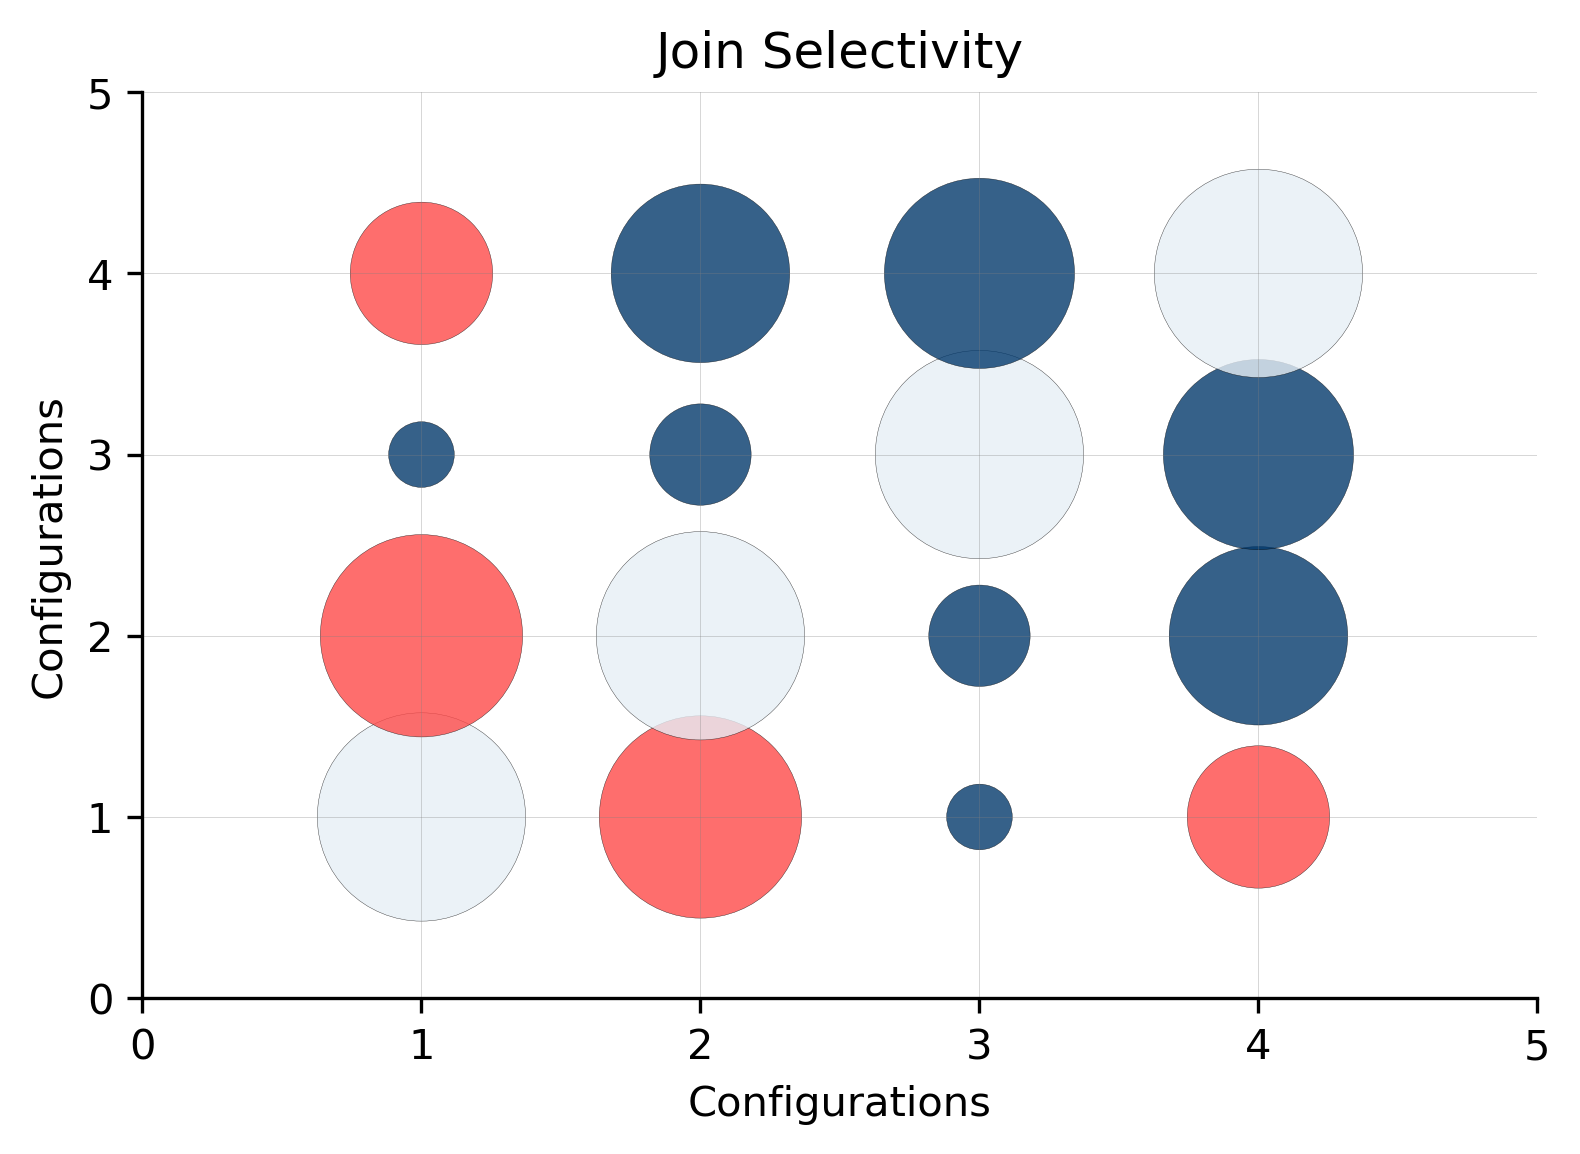
\includegraphics[width=0.48\columnwidth]{figures/join_selectivity_10k_bubble.png}
      \label{fig:js3}
    }
    \qquad
    \subfloat[Dataset 50K]{
      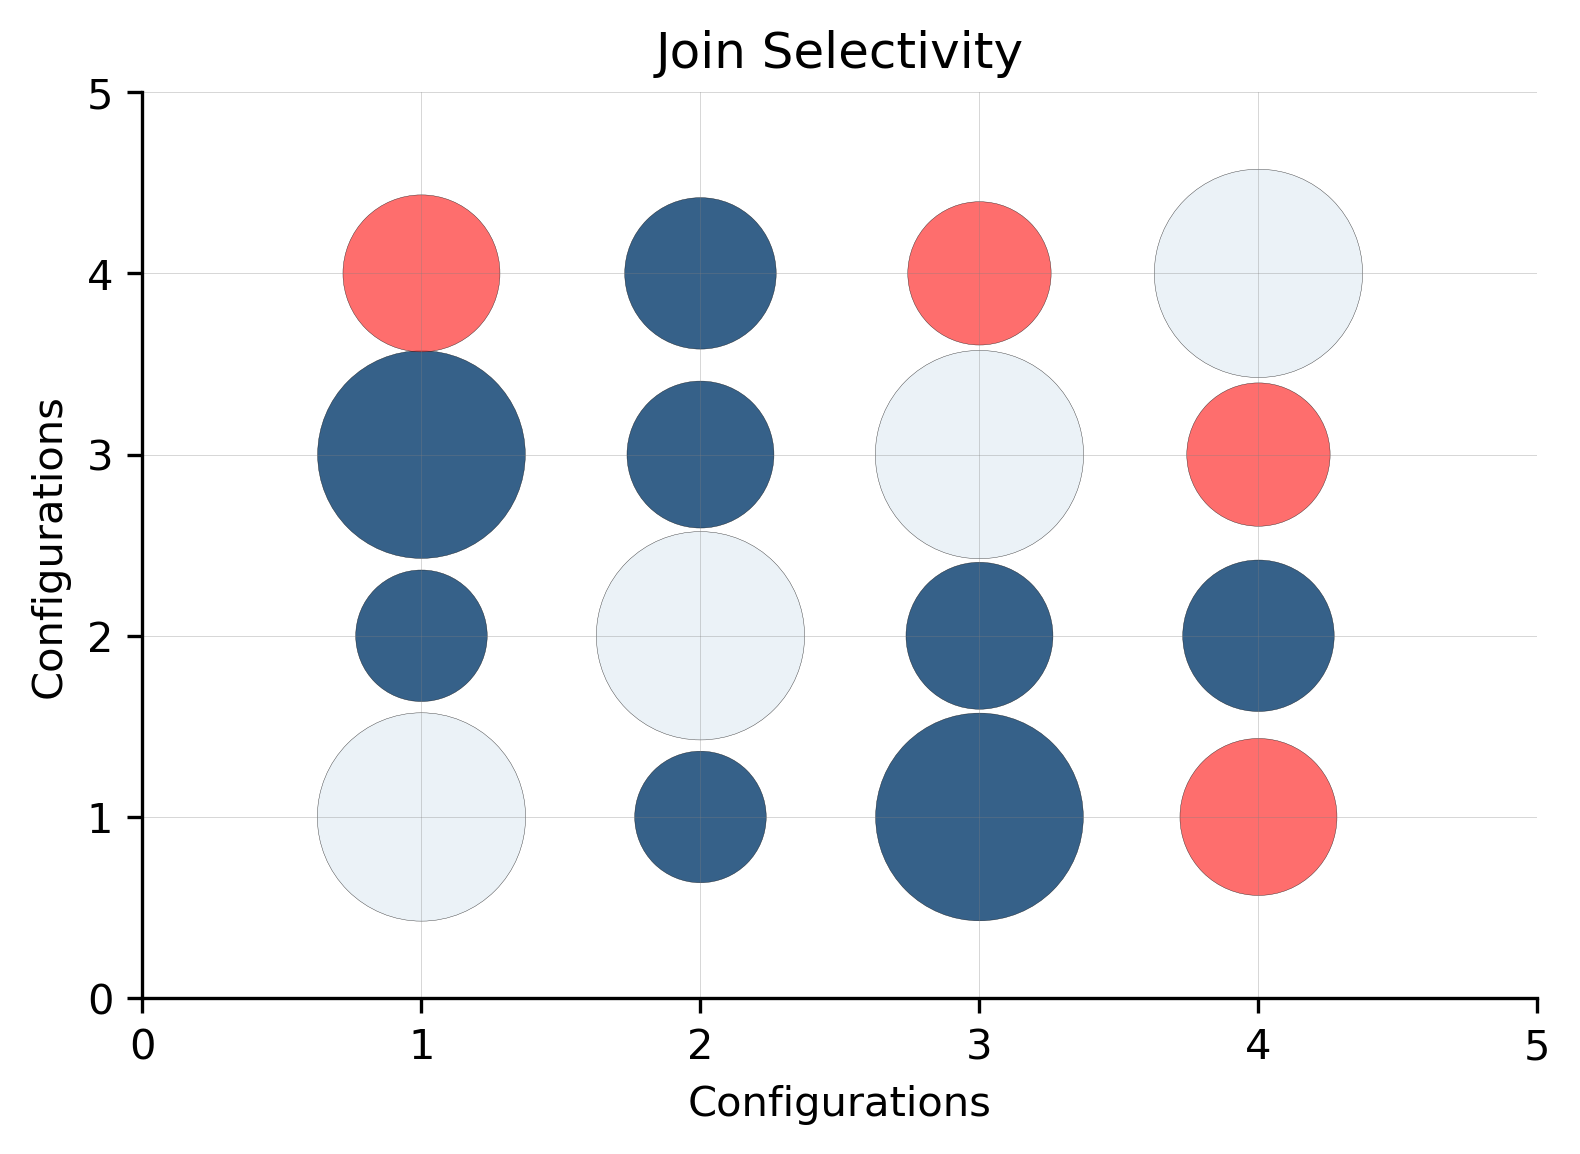
\includegraphics[width=0.48\columnwidth]{figures/join_selectivity_50k_bubble.png}
      \label{fig:naive4}
    }
    \subfloat[Combination of 1K, 10K, and 50K]{
      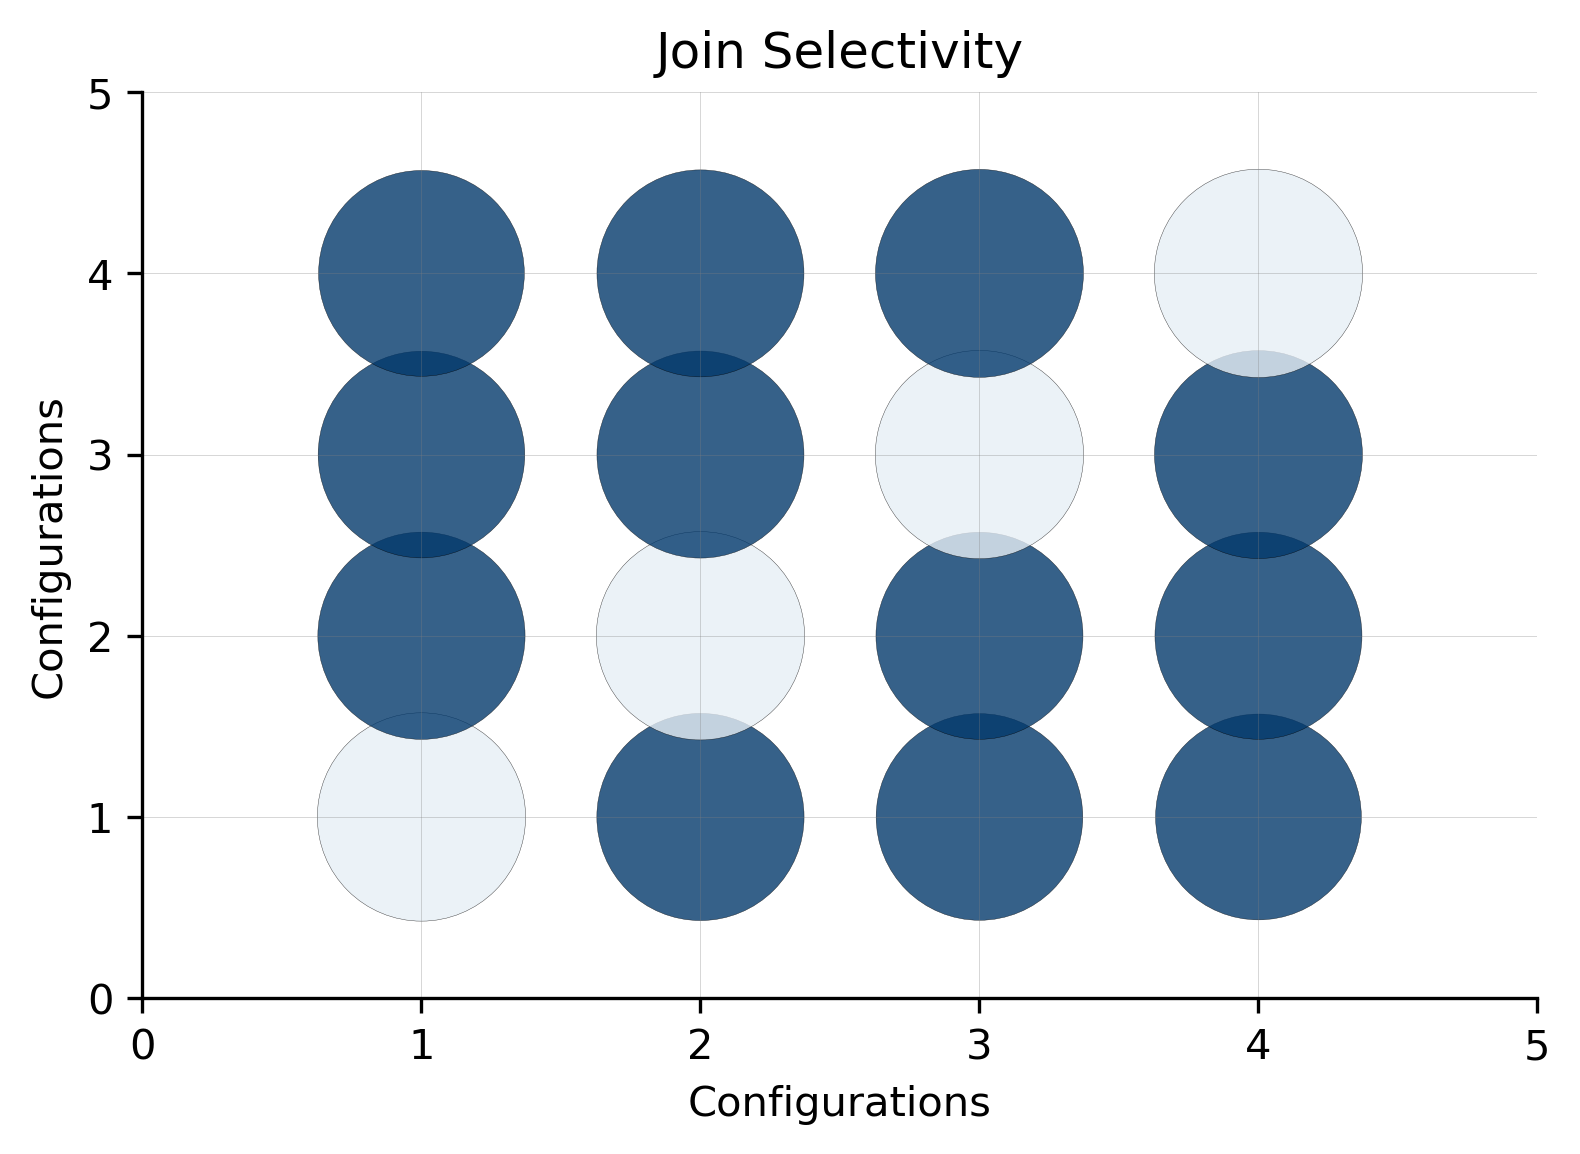
\includegraphics[width=0.48\columnwidth]{figures/join_selectivity_allk_bubble.png}
      \label{fig:js4}
    }
    \caption[Knowledge Graph Tools on Join Selectivity]{\textbf{Comparison of Knowledge Graph Tools on Join Selectivity.} The first two configurations, i.e., 1-2 on x- and y-axis represent SDM-RDFizer on joins with \textit{high} selectivity (5\%-20\% of data) and joins with \textit{low} selectivity (60\%-100\% of data), respectively.  Configurations 3 and 4 represent RMLMapper on joins with \textit{high} selectivity (5\%-20\% of data) and joins with \textit{low} selectivity (60\%-100\% of data), respectively. Grey bubbles correspond to correlation value of $1.0$; blue bubbles show a positive correlation while red bubbles show a negative correlation. Dataset size and join selectivity affect both engines differently.}
    \label{fig:joinselectivity_bubble}
\end{figure}



\noindent \textbf{Relation Types:}
Figure~\ref{fig:relation_type_bubble} reports on the correlation of different configurations for various join relation types. We can observe in Figures \ref{fig:rt_1k}, \ref{fig:rt_10k}, and \ref{fig:rt_50k} several red bubbles, indicating a negative correlation in the behavior of the compared configurations and engines. Contrary, Figure \ref{fig:rt_all} does not depict any red bubble, suggesting thus, that the two engines in all the configurations exhibit the same behavior. These results clearly illustrate the need of considering different configurations and parameters in order to avoid drawing wrong conclusions about the main characteristics of existing tools. 


\noindent \textbf{Join Duplicates:}
Figure~\ref{fig:duplicates_bubble} depicts the correlation between different configurations when different setting of duplicates are produced during the execution of joins between triple maps. As can be observed, Figures \ref{fig:naive1}, and \ref{fig:naive2} include several red bubbles that indicate an opposite behavior of the engines. Contrary, Figures \ref{fig:js0}, and \ref{fig:js1} suggest that both engines behave similarly. 


\noindent \textbf{Join Selectivity:}
Figure~\ref{fig:joinselectivity_bubble} shows the correlation between different configurations for the selectivity of join conditions. Similarly, these testbeds reveal contradicting patterns in the behaviors of the studied engines. On one hand, Figures \ref{fig:naive3}, \ref{fig:js3}, and \ref{fig:naive4} are composed of several red bubbles and indicate that these engines perform differently whenever the selectivity of the join condition is changed. Surprisingly,  when the size of these datasets are also taken into account in the testbed (Figure \ref{fig:js4}), these patterns are hidden, and the results of the evaluation suggest that both engines perform similarly whenever the selectivity of the join condition is changed. 

The results reported in this experimental study provide clear evidence of the importance of the variables and configurations that composed the methodology devised in this work. Actually, in the four studied cases, they reveal important patterns that could not be observed whenever other parameters were studied simultaneously. Based on these observations, we can conclude that these variables and configurations should be included in the benchmarks in order to ensure that the characteristics of knowledge graph creation engines are uncovered. Thus, these observations allow us to answer our three research questions: \textbf{RQ1}, \textbf{RQ2}, and \textbf{RQ3}. We encourage developers and users of knowledge graph creation tools to bear in mind them during benchmarking in order to draw clear conclusions about the performance of their tools.


\subsection{Conclusions}
In this section, we performed an in-depth analysis of the variables and configurations that impact on the behavior of two engines. The observation that existing engines exhibit heterogeneous behaviors whenever small changes in the testbeds are conducted, motivated the need of conducting this study involving a set of parameters that can reveal patterns in the behavior of the studied engines. Additionally, the lack of testbeds encouraged us to acquit the definition of variables and configurations that enable for the characterization of the pitfalls of existing engines and for identifying the list of challenges and research directions in the state of the art. 
With the proposed analysis and the results of the experimental study, we contribute with an empirical configuration that can be reused for the evaluation of other knowledge graph creation tools and mapping languages (e.g., SPARQL-Generate, TARQL, or R2RML). Furthermore, our set of variables and configurations can be utilized as a guideline during testing and benchmarking. One of the main lessons learned during the definition and evaluation of our approach, is that none of the evaluated engines behaves consistently whenever the complexity of the testbeds increases. Our ambition is that the reported results inspire the community to define general testbeds that facilitate the understanding of the state of the art and the development of novel tools for the creation of knowledge graphs at large scale.  In the future, we plan to define testbeds and conduct a more detailed analysis of other engines and mapping languages. Moreover, we envision to motivate the community to conduct a joint effort in the definition of benchmarks that enable for fair evaluations of knowledge graph creation tools with replicable and generalizable results. 
